\documentclass[a4paper,fleqn]{cas-dc}
\input{glyphtounicode}
\pdfgentounicode=1
\usepackage[authoryear]{natbib}
\usepackage{array}
\usepackage{enumitem}
\usepackage{orcidlink}
\usepackage{placeins}
\usepackage{silence}
\WarningFilter{hyperref}{Ignoring empty anchor}


\emergencystretch=3em
\hbadness=10000

\newcommand{\sigstar}{\textsuperscript{*}}
\newcommand{\AP}{\mathrm{AP}}
\newcommand{\Jclean}{\mathrm{J95}}
% Generated by analysis/build_nn_tables.py from nn_final_stats.json
\newcommand{\nnActClsAmaxMaxCoco}{815}
\newcommand{\nnActClsAmaxMaxKitti}{6156}
\newcommand{\nnActClsAmaxMaxVoc}{1116}
\newcommand{\nnActClsAmaxMedCoco}{7.5}
\newcommand{\nnActClsAmaxMedKitti}{10.3}
\newcommand{\nnActClsAmaxMedVoc}{8.3}
\newcommand{\nnActClsKurtMaxCoco}{21296}
\newcommand{\nnActClsKurtMaxKitti}{21826}
\newcommand{\nnActClsKurtMaxVoc}{62412}
\newcommand{\nnActClsKurtMedCoco}{2.8}
\newcommand{\nnActClsKurtMedKitti}{3.1}
\newcommand{\nnActClsKurtMedVoc}{2.5}
\newcommand{\nnActClsKurtTailCoco}{6.5}
\newcommand{\nnActClsKurtTailKitti}{9.1}
\newcommand{\nnActClsKurtTailVoc}{6.7}
\newcommand{\nnActRegAmaxMaxCoco}{1282}
\newcommand{\nnActRegAmaxMaxKitti}{7491}
\newcommand{\nnActRegAmaxMaxVoc}{2290}
\newcommand{\nnActRegAmaxMedCoco}{7.6}
\newcommand{\nnActRegAmaxMedKitti}{8.6}
\newcommand{\nnActRegAmaxMedVoc}{9.3}
\newcommand{\nnActRegKurtMaxCoco}{313956}
\newcommand{\nnActRegKurtMaxKitti}{204795}
\newcommand{\nnActRegKurtMaxVoc}{261078}
\newcommand{\nnActRegKurtMedCoco}{6.0}
\newcommand{\nnActRegKurtMedKitti}{10.6}
\newcommand{\nnActRegKurtMedVoc}{8.0}
\newcommand{\nnActRegKurtTailCoco}{40.3}
\newcommand{\nnActRegKurtTailKitti}{43.6}
\newcommand{\nnActRegKurtTailVoc}{52.9}
\newcommand{\nnActStaticClsMaxCoco}{21.9}
\newcommand{\nnActStaticClsMaxKitti}{54.1}
\newcommand{\nnActStaticClsMaxVoc}{15.5}
\newcommand{\nnActStaticClsMedCoco}{8.5}
\newcommand{\nnActStaticClsMedKitti}{12.5}
\newcommand{\nnActStaticClsMedVoc}{9.1}
\newcommand{\nnActStaticRegMaxCoco}{57.5}
\newcommand{\nnActStaticRegMaxKitti}{97.5}
\newcommand{\nnActStaticRegMaxVoc}{90.4}
\newcommand{\nnActStaticRegMedCoco}{25.4}
\newcommand{\nnActStaticRegMedKitti}{25.3}
\newcommand{\nnActStaticRegMedVoc}{31.6}
\newcommand{\nnArmFeCleanKitti}{49.48}
\newcommand{\nnArmFeCleanVoc}{56.17}
\newcommand{\nnArmFeJKitti}{49.25}
\newcommand{\nnArmFeJVoc}{56.21}
\newcommand{\nnArmFeLegacyCleanKitti}{49.19}
\newcommand{\nnArmFeLegacyCleanVoc}{56.17}
\newcommand{\nnArmFpCleanKitti}{50.15}
\newcommand{\nnArmFpCleanVoc}{57.23}
\newcommand{\nnArmInCleanKitti}{28.29}
\newcommand{\nnArmInCleanVoc}{53.30}
\newcommand{\nnArmInJKitti}{28.18}
\newcommand{\nnArmInJVoc}{53.18}
\newcommand{\nnArmLegacyCleanKitti}{7.21}
\newcommand{\nnArmLegacyCleanVoc}{33.61}
\newcommand{\nnArmSelCleanKitti}{49.60}
\newcommand{\nnArmSelCleanVoc}{55.87}
\newcommand{\nnArmSelJKitti}{49.53}
\newcommand{\nnArmSelJVoc}{55.79}
\newcommand{\nnCcCKitti}{$+1.34$~$[+1.17,+1.48]$}
\newcommand{\nnCcCKittiP}{+1.34}
\newcommand{\nnCcCVoc}{$+0.64$~$[+0.52,+0.76]$}
\newcommand{\nnCcCVocP}{+0.64}
\newcommand{\nnCcDHKitti}{$-0.50$~$[-1.01,+0.03]$}
\newcommand{\nnCcDHKittiP}{-0.50}
\newcommand{\nnCcDHVoc}{$-0.71$~$[-1.02,-0.39]$}
\newcommand{\nnCcDHVocP}{-0.71}
\newcommand{\nnCcDIKitti}{$+0.05$~$[-0.54,+0.59]$}
\newcommand{\nnCcDIKittiP}{+0.05}
\newcommand{\nnCcDIVoc}{$+0.54$~$[+0.24,+0.88]$}
\newcommand{\nnCcDIVocP}{+0.54}
\newcommand{\nnCcFCKitti}{$-15.04$~$[-15.96,-14.17]$}
\newcommand{\nnCcFCKittiP}{-15.04}
\newcommand{\nnCcFCVoc}{$-2.13$~$[-2.30,-1.97]$}
\newcommand{\nnCcFCVocP}{-2.13}
\newcommand{\nnCcFDHKitti}{$+6.17$~$[+5.12,+7.10]$}
\newcommand{\nnCcFDHKittiP}{+6.17}
\newcommand{\nnCcFDHVoc}{$+0.18$~$[-0.12,+0.50]$}
\newcommand{\nnCcFDHVocP}{+0.18}
\newcommand{\nnCcFDIKitti}{$+2.77$~$[+1.98,+3.48]$}
\newcommand{\nnCcFDIKittiP}{+2.77}
\newcommand{\nnCcFDIVoc}{$+0.17$~$[-0.10,+0.49]$}
\newcommand{\nnCcFDIVocP}{+0.17}
\newcommand{\nnCcFHKitti}{$-13.34$~$[-14.13,-12.57]$}
\newcommand{\nnCcFHKittiP}{-13.34}
\newcommand{\nnCcFHVoc}{$-2.12$~$[-2.32,-1.96]$}
\newcommand{\nnCcFHVocP}{-2.12}
\newcommand{\nnCcFHxKitti}{$-15.65$~$[-16.58,-14.74]$}
\newcommand{\nnCcFHxKittiP}{-15.65}
\newcommand{\nnCcFHxVoc}{$-2.37$~$[-2.60,-2.18]$}
\newcommand{\nnCcFHxVocP}{-2.37}
\newcommand{\nnCcFInKitti}{$-16.74$~$[-17.85,-15.66]$}
\newcommand{\nnCcFInKittiP}{-16.74}
\newcommand{\nnCcFInVoc}{$-2.13$~$[-2.33,-1.93]$}
\newcommand{\nnCcFInVocP}{-2.13}
\newcommand{\nnCcFJKitti}{$-19.51$~$[-20.90,-18.04]$}
\newcommand{\nnCcFJKittiP}{-19.51}
\newcommand{\nnCcFJVoc}{$-2.31$~$[-2.68,-1.98]$}
\newcommand{\nnCcFJVocP}{-2.31}
\newcommand{\nnCcHKitti}{$+1.07$~$[+0.87,+1.26]$}
\newcommand{\nnCcHKittiP}{+1.07}
\newcommand{\nnCcHVoc}{$+0.02$~$[-0.13,+0.16]$}
\newcommand{\nnCcHVocP}{+0.02}
\newcommand{\nnCcHxKitti}{$+1.27$~$[+1.06,+1.50]$}
\newcommand{\nnCcHxKittiP}{+1.27}
\newcommand{\nnCcHxVoc}{$+0.07$~$[-0.10,+0.23]$}
\newcommand{\nnCcHxVocP}{+0.07}
\newcommand{\nnCcInKitti}{$+1.61$~$[+1.37,+1.79]$}
\newcommand{\nnCcInKittiP}{+1.61}
\newcommand{\nnCcInVoc}{$+1.27$~$[+1.12,+1.42]$}
\newcommand{\nnCcInVocP}{+1.27}
\newcommand{\nnCcJKitti}{$+1.56$~$[+1.02,+2.10]$}
\newcommand{\nnCcJKittiP}{+1.56}
\newcommand{\nnCcJVoc}{$+0.73$~$[+0.40,+1.01]$}
\newcommand{\nnCcJVocP}{+0.73}
\newcommand{\nnCcQCKitti}{$+1.29$~$[+1.08,+1.45]$}
\newcommand{\nnCcQCKittiP}{+1.29}
\newcommand{\nnCcQCVoc}{$+0.81$~$[+0.70,+0.93]$}
\newcommand{\nnCcQCVocP}{+0.81}
\newcommand{\nnCcQDHKitti}{$-0.94$~$[-1.60,-0.33]$}
\newcommand{\nnCcQDHKittiP}{-0.94}
\newcommand{\nnCcQDHVoc}{$-0.39$~$[-0.69,-0.07]$}
\newcommand{\nnCcQDHVocP}{-0.39}
\newcommand{\nnCcQDIKitti}{$-0.26$~$[-0.89,+0.30]$}
\newcommand{\nnCcQDIKittiP}{-0.26}
\newcommand{\nnCcQDIVoc}{$+0.98$~$[+0.70,+1.31]$}
\newcommand{\nnCcQDIVocP}{+0.98}
\newcommand{\nnCcQHKitti}{$+0.95$~$[+0.73,+1.15]$}
\newcommand{\nnCcQHKittiP}{+0.95}
\newcommand{\nnCcQHVoc}{$+0.13$~$[-0.02,+0.28]$}
\newcommand{\nnCcQHVocP}{+0.13}
\newcommand{\nnCcQHxKitti}{$+1.20$~$[+0.93,+1.43]$}
\newcommand{\nnCcQHxKittiP}{+1.20}
\newcommand{\nnCcQHxVoc}{$+0.21$~$[+0.04,+0.38]$}
\newcommand{\nnCcQHxVocP}{+0.21}
\newcommand{\nnCcQInKitti}{$+1.64$~$[+1.33,+1.86]$}
\newcommand{\nnCcQInKittiP}{+1.64}
\newcommand{\nnCcQInVoc}{$+1.50$~$[+1.35,+1.66]$}
\newcommand{\nnCcQInVocP}{+1.50}
\newcommand{\nnCcQJKitti}{$+1.90$~$[+1.28,+2.54]$}
\newcommand{\nnCcQJKittiP}{+1.90}
\newcommand{\nnCcQJVoc}{$+0.52$~$[+0.22,+0.80]$}
\newcommand{\nnCcQJVocP}{+0.52}
\newcommand{\nnCpArmFeCFco}{27.51}
\newcommand{\nnCpArmFeCRet}{30.58}
\newcommand{\nnCpArmFeJFco}{34.24}
\newcommand{\nnCpArmFeJRet}{37.84}
\newcommand{\nnCpArmFpCFco}{27.61}
\newcommand{\nnCpArmFpCRet}{31.18}
\newcommand{\nnCpArmFpJFco}{34.32}
\newcommand{\nnCpArmFpJRet}{38.30}
\newcommand{\nnCpArmInCFco}{27.44}
\newcommand{\nnCpArmInCRet}{27.97}
\newcommand{\nnCpArmInJFco}{34.19}
\newcommand{\nnCpArmInJRet}{34.70}
\newcommand{\nnCpArmSelCFco}{27.45}
\newcommand{\nnCpArmSelCRet}{29.91}
\newcommand{\nnCpArmSelJFco}{34.20}
\newcommand{\nnCpArmSelJRet}{37.27}
\newcommand{\nnCpFmDEFco}{$+0.02$~$[-0.20,+0.28]$}
\newcommand{\nnCpFmDEPFco}{+0.02}
\newcommand{\nnCpFmDEPRet}{-0.53}
\newcommand{\nnCpFmDERet}{$-0.53$~$[-0.90,-0.14]$}
\newcommand{\nnCpFmHDEFco}{$+0.04$~$[-0.12,+0.26]$}
\newcommand{\nnCpFmHDEPFco}{+0.04}
\newcommand{\nnCpFmHDEPRet}{-0.39}
\newcommand{\nnCpFmHDERet}{$-0.39$~$[-0.74,-0.07]$}
\newcommand{\nnCpFmHJFco}{$+0.14$~$[-0.09,+0.31]$}
\newcommand{\nnCpFmHJPFco}{+0.14}
\newcommand{\nnCpFmHJPRet}{+3.60}
\newcommand{\nnCpFmHJRet}{$+3.60$~$[+3.28,+4.05]$}
\newcommand{\nnCpFmJFco}{$+0.05$~$[-0.22,+0.27]$}
\newcommand{\nnCpFmJPFco}{+0.05}
\newcommand{\nnCpFmJPRet}{+3.14}
\newcommand{\nnCpFmJRet}{$+3.14$~$[+2.78,+3.57]$}
\newcommand{\nnCpFpDEFco}{$+0.04$~$[-0.11,+0.25]$}
\newcommand{\nnCpFpDEPFco}{+0.04}
\newcommand{\nnCpFpDEPRet}{+0.25}
\newcommand{\nnCpFpDERet}{$+0.25$~$[-0.07,+0.53]$}
\newcommand{\nnCpFpJFco}{$+0.13$~$[-0.11,+0.29]$}
\newcommand{\nnCpFpJPFco}{+0.13}
\newcommand{\nnCpFpJPRet}{+1.03}
\newcommand{\nnCpFpJRet}{$+1.03$~$[+0.74,+1.39]$}
\newcommand{\nnCpFsDEFco}{$+0.02$~$[-0.19,+0.27]$}
\newcommand{\nnCpFsDEPFco}{+0.02}
\newcommand{\nnCpFsDEPRet}{+0.11}
\newcommand{\nnCpFsDERet}{$+0.11$~$[-0.28,+0.48]$}
\newcommand{\nnCpFsJFco}{$+0.04$~$[-0.21,+0.24]$}
\newcommand{\nnCpFsJPFco}{+0.04}
\newcommand{\nnCpFsJPRet}{+0.56}
\newcommand{\nnCpFsJRet}{$+0.56$~$[+0.22,+0.96]$}
\newcommand{\nnCpRecovFco}{23}
\newcommand{\nnCpRecovRet}{82}
\newcommand{\nnCpSmDEFco}{$0.00$~$[-0.07,+0.07]$}
\newcommand{\nnCpSmDEPFco}{0.00}
\newcommand{\nnCpSmDEPRet}{-0.64}
\newcommand{\nnCpSmDERet}{$-0.64$~$[-0.84,-0.42]$}
\newcommand{\nnCpSmJFco}{$+0.01$~$[-0.06,+0.09]$}
\newcommand{\nnCpSmJPFco}{+0.01}
\newcommand{\nnCpSmJPRet}{+2.58}
\newcommand{\nnCpSmJRet}{$+2.58$~$[+2.33,+2.85]$}
\newcommand{\nnCtCKitti}{$-1.69$~$[-1.88,-1.44]$}
\newcommand{\nnCtCKittiP}{-1.69}
\newcommand{\nnCtCVoc}{$+1.26$~$[+1.15,+1.37]$}
\newcommand{\nnCtCVocP}{+1.26}
\newcommand{\nnCtDHKitti}{$+0.69$~$[-0.10,+1.37]$}
\newcommand{\nnCtDHKittiP}{+0.69}
\newcommand{\nnCtDHVoc}{$+0.62$~$[+0.30,+0.96]$}
\newcommand{\nnCtDHVocP}{+0.62}
\newcommand{\nnCtDIKitti}{$+1.36$~$[+0.61,+2.16]$}
\newcommand{\nnCtDIKittiP}{+1.36}
\newcommand{\nnCtDIVoc}{$-0.19$~$[-0.49,+0.13]$}
\newcommand{\nnCtDIVocP}{-0.19}
\newcommand{\nnCtFCKitti}{$-18.07$~$[-19.07,-17.00]$}
\newcommand{\nnCtFCKittiP}{-18.07}
\newcommand{\nnCtFCVoc}{$-1.51$~$[-1.68,-1.35]$}
\newcommand{\nnCtFCVocP}{-1.51}
\newcommand{\nnCtFDHKitti}{$+3.41$~$[+2.51,+4.23]$}
\newcommand{\nnCtFDHKittiP}{+3.41}
\newcommand{\nnCtFDHVoc}{$+0.25$~$[-0.04,+0.57]$}
\newcommand{\nnCtFDHVocP}{+0.25}
\newcommand{\nnCtFDIKitti}{$+8.02$~$[+7.05,+8.94]$}
\newcommand{\nnCtFDIKittiP}{+8.02}
\newcommand{\nnCtFDIVoc}{$+0.70$~$[+0.41,+1.01]$}
\newcommand{\nnCtFDIVocP}{+0.70}
\newcommand{\nnCtFHKitti}{$-20.37$~$[-21.58,-19.14]$}
\newcommand{\nnCtFHKittiP}{-20.37}
\newcommand{\nnCtFHVoc}{$-1.74$~$[-1.94,-1.53]$}
\newcommand{\nnCtFHVocP}{-1.74}
\newcommand{\nnCtFInKitti}{$-15.76$~$[-16.63,-14.86]$}
\newcommand{\nnCtFInKittiP}{-15.76}
\newcommand{\nnCtFInVoc}{$-1.28$~$[-1.47,-1.12]$}
\newcommand{\nnCtFInVocP}{-1.28}
\newcommand{\nnCtFJKitti}{$-23.78$~$[-25.30,-22.13]$}
\newcommand{\nnCtFJKittiP}{-23.78}
\newcommand{\nnCtFJVoc}{$-1.99$~$[-2.34,-1.66]$}
\newcommand{\nnCtFJVocP}{-1.99}
\newcommand{\nnCtHKitti}{$-2.02$~$[-2.31,-1.73]$}
\newcommand{\nnCtHKittiP}{-2.02}
\newcommand{\nnCtHVoc}{$+1.66$~$[+1.52,+1.83]$}
\newcommand{\nnCtHVocP}{+1.66}
\newcommand{\nnCtInKitti}{$-1.35$~$[-1.56,-1.04]$}
\newcommand{\nnCtInKittiP}{-1.35}
\newcommand{\nnCtInVoc}{$+0.86$~$[+0.72,+0.99]$}
\newcommand{\nnCtInVocP}{+0.86}
\newcommand{\nnCtJKitti}{$-2.71$~$[-3.38,-1.93]$}
\newcommand{\nnCtJKittiP}{-2.71}
\newcommand{\nnCtJVoc}{$+1.04$~$[+0.72,+1.34]$}
\newcommand{\nnCtJVocP}{+1.04}
\newcommand{\nnCtQCKitti}{$-1.73$~$[-1.96,-1.47]$}
\newcommand{\nnCtQCKittiP}{-1.73}
\newcommand{\nnCtQCVoc}{$+1.43$~$[+1.32,+1.55]$}
\newcommand{\nnCtQCVocP}{+1.43}
\newcommand{\nnCtQDHKitti}{$+0.37$~$[-0.28,+0.90]$}
\newcommand{\nnCtQDHKittiP}{+0.37}
\newcommand{\nnCtQDHVoc}{$+1.06$~$[+0.76,+1.38]$}
\newcommand{\nnCtQDHVocP}{+1.06}
\newcommand{\nnCtQDIKitti}{$+0.91$~$[+0.28,+1.47]$}
\newcommand{\nnCtQDIKittiP}{+0.91}
\newcommand{\nnCtQDIVoc}{$+0.13$~$[-0.15,+0.43]$}
\newcommand{\nnCtQDIVocP}{+0.13}
\newcommand{\nnCtQHKitti}{$-2.00$~$[-2.32,-1.69]$}
\newcommand{\nnCtQHKittiP}{-2.00}
\newcommand{\nnCtQHVoc}{$+1.89$~$[+1.75,+2.06]$}
\newcommand{\nnCtQHVocP}{+1.89}
\newcommand{\nnCtQInKitti}{$-1.47$~$[-1.68,-1.18]$}
\newcommand{\nnCtQInKittiP}{-1.47}
\newcommand{\nnCtQInVoc}{$+0.97$~$[+0.82,+1.12]$}
\newcommand{\nnCtQInVocP}{+0.97}
\newcommand{\nnCtQJKitti}{$-2.37$~$[-2.90,-1.74]$}
\newcommand{\nnCtQJKittiP}{-2.37}
\newcommand{\nnCtQJVoc}{$+0.84$~$[+0.54,+1.12]$}
\newcommand{\nnCtQJVocP}{+0.84}
\newcommand{\nnDECocoM}{+0.60}
\newcommand{\nnDECocoN}{-0.32}
\newcommand{\nnDECocoX}{-0.53}
\newcommand{\nnDEKittiM}{-0.68}
\newcommand{\nnDEKittiN}{-0.01}
\newcommand{\nnDEKittiX}{-0.69}
\newcommand{\nnDEVocM}{-0.57}
\newcommand{\nnDEVocN}{+0.31}
\newcommand{\nnDEVocX}{+0.14}
\newcommand{\nnDEciCocoM}{$+0.60$~$[+0.27,+0.97]$}
\newcommand{\nnDEciCocoN}{$-0.32$~$[-0.67,+0.01]$}
\newcommand{\nnDEciCocoX}{$-0.53$~$[-0.93,-0.18]$}
\newcommand{\nnDEciKittiM}{$-0.68$~$[-1.32,-0.05]$}
\newcommand{\nnDEciKittiN}{$-0.01$~$[-0.67,+0.91]$}
\newcommand{\nnDEciKittiX}{$-0.69$~$[-1.13,-0.33]$}
\newcommand{\nnDEciVocM}{$-0.57$~$[-0.80,-0.34]$}
\newcommand{\nnDEciVocN}{$+0.31$~$[+0.07,+0.59]$}
\newcommand{\nnDEciVocX}{$+0.14$~$[-0.07,+0.36]$}
\newcommand{\nnDEexCocoM}{+0.60}
\newcommand{\nnDEexCocoN}{-0.28}
\newcommand{\nnDEexCocoX}{-0.59}
\newcommand{\nnDEexKittiM}{-0.35}
\newcommand{\nnDEexKittiN}{+0.15}
\newcommand{\nnDEexKittiX}{-0.65}
\newcommand{\nnDEexVocM}{-0.53}
\newcommand{\nnDEexVocN}{+0.34}
\newcommand{\nnDEexVocX}{+0.13}
\newcommand{\nnDiagBackboneJ}{49.14}
\newcommand{\nnDiagClsJ}{50.57}
\newcommand{\nnDiagConvAddJ}{15.75}
\newcommand{\nnDiagFpEightDeficitJ}{41.8}
\newcommand{\nnDiagFpEightJ}{48.50}
\newcommand{\nnDiagFpThirtyTwoJ}{50.44}
\newcommand{\nnDiagHeadsJ}{17.09}
\newcommand{\nnDiagLegacyJ}{6.72}
\newcommand{\nnDiagMatchedFiveJ}{28.18}
\newcommand{\nnDiagMatchedJ}{27.91}
\newcommand{\nnDiagMaxJ}{23.94}
\newcommand{\nnDiagNoRegJ}{49.50}
\newcommand{\nnDiagPreprocGain}{21.2}
\newcommand{\nnDiagRegJ}{16.41}
\newcommand{\nnDiagSharedMaskJ}{28.74}
\newcommand{\nnFamCocoMFog}{+0.36}
\newcommand{\nnFamCocoMGn}{-0.36}
\newcommand{\nnFamCocoMJpeg}{+1.43}
\newcommand{\nnFamCocoMMb}{+0.99}
\newcommand{\nnFamCocoNFog}{+0.17}
\newcommand{\nnFamCocoNGn}{-0.22}
\newcommand{\nnFamCocoNJpeg}{-0.56}
\newcommand{\nnFamCocoNMb}{-0.69}
\newcommand{\nnFamCocoXFog}{+0.15}
\newcommand{\nnFamCocoXGn}{-0.28}
\newcommand{\nnFamCocoXJpeg}{-2.10}
\newcommand{\nnFamCocoXMb}{+0.13}
\newcommand{\nnFamKittiMFog}{+0.38}
\newcommand{\nnFamKittiMGn}{-0.44}
\newcommand{\nnFamKittiMJpeg}{+0.02}
\newcommand{\nnFamKittiMMb}{-2.68}
\newcommand{\nnFamKittiNFog}{+1.11}
\newcommand{\nnFamKittiNGn}{+0.41}
\newcommand{\nnFamKittiNJpeg}{+0.17}
\newcommand{\nnFamKittiNMb}{-1.71}
\newcommand{\nnFamKittiXFog}{-0.40}
\newcommand{\nnFamKittiXGn}{-1.98}
\newcommand{\nnFamKittiXJpeg}{-0.43}
\newcommand{\nnFamKittiXMb}{+0.03}
\newcommand{\nnFamSDpFog}{0.4}
\newcommand{\nnFamSDpGn}{0.7}
\newcommand{\nnFamSDpJpeg}{1.0}
\newcommand{\nnFamSDpMb}{1.1}
\newcommand{\nnFamSDsFog}{0.4}
\newcommand{\nnFamSDsGn}{0.8}
\newcommand{\nnFamSDsJpeg}{1.0}
\newcommand{\nnFamSDsMb}{1.2}
\newcommand{\nnFamVocMFog}{-0.03}
\newcommand{\nnFamVocMGn}{-0.48}
\newcommand{\nnFamVocMJpeg}{-1.23}
\newcommand{\nnFamVocMMb}{-0.56}
\newcommand{\nnFamVocNFog}{+0.35}
\newcommand{\nnFamVocNGn}{+0.28}
\newcommand{\nnFamVocNJpeg}{+0.27}
\newcommand{\nnFamVocNMb}{+0.34}
\newcommand{\nnFamVocXFog}{+0.26}
\newcommand{\nnFamVocXGn}{+0.69}
\newcommand{\nnFamVocXJpeg}{-1.07}
\newcommand{\nnFamVocXMb}{+0.67}
\newcommand{\nnFcosArmFeCKitti}{33.32}
\newcommand{\nnFcosArmFeCVoc}{34.51}
\newcommand{\nnFcosArmFeJKitti}{47.06}
\newcommand{\nnFcosArmFeJVoc}{48.88}
\newcommand{\nnFcosArmFpCKitti}{33.95}
\newcommand{\nnFcosArmFpCVoc}{34.88}
\newcommand{\nnFcosArmFpJKitti}{47.60}
\newcommand{\nnFcosArmFpJVoc}{49.22}
\newcommand{\nnFcosArmInCKitti}{33.82}
\newcommand{\nnFcosArmInCVoc}{34.59}
\newcommand{\nnFcosArmInJKitti}{47.53}
\newcommand{\nnFcosArmInJVoc}{49.02}
\newcommand{\nnFcosArmSelCKitti}{33.82}
\newcommand{\nnFcosArmSelCVoc}{34.58}
\newcommand{\nnFcosArmSelJKitti}{47.53}
\newcommand{\nnFcosArmSelJVoc}{49.04}
\newcommand{\nnFcosFmCKitti}{$-0.50$~$[-0.66,-0.36]$}
\newcommand{\nnFcosFmCPKitti}{-0.50}
\newcommand{\nnFcosFmCPVoc}{-0.08}
\newcommand{\nnFcosFmCVoc}{$-0.08$~$[-0.15,-0.01]$}
\newcommand{\nnFcosFmDEKitti}{$-0.04$~$[-0.44,+0.40]$}
\newcommand{\nnFcosFmDEPKitti}{-0.04}
\newcommand{\nnFcosFmDEPVoc}{+0.07}
\newcommand{\nnFcosFmDEVoc}{$+0.07$~$[-0.13,+0.25]$}
\newcommand{\nnFcosFmJKitti}{$-0.47$~$[-0.990,-0.001]$}
\newcommand{\nnFcosFmJPKitti}{-0.47}
\newcommand{\nnFcosFmJPVoc}{-0.14}
\newcommand{\nnFcosFmJVoc}{$-0.14$~$[-0.33,+0.07]$}
\newcommand{\nnFcosFpCKitti}{$+0.12$~$[+0.01,+0.22]$}
\newcommand{\nnFcosFpCPKitti}{+0.12}
\newcommand{\nnFcosFpCPVoc}{+0.30}
\newcommand{\nnFcosFpCVoc}{$+0.30$~$[+0.26,+0.36]$}
\newcommand{\nnFcosFpDEKitti}{$+0.05$~$[-0.29,+0.35]$}
\newcommand{\nnFcosFpDEPKitti}{+0.05}
\newcommand{\nnFcosFpDEPVoc}{+0.12}
\newcommand{\nnFcosFpDEVoc}{$+0.12$~$[-0.03,+0.27]$}
\newcommand{\nnFcosFpJKitti}{$+0.07$~$[-0.25,+0.42]$}
\newcommand{\nnFcosFpJPKitti}{+0.07}
\newcommand{\nnFcosFpJPVoc}{+0.19}
\newcommand{\nnFcosFpJVoc}{$+0.19$~$[+0.04,+0.34]$}
\newcommand{\nnFcosFsCKitti}{$-0.50$~$[-0.66,-0.35]$}
\newcommand{\nnFcosFsCPKitti}{-0.50}
\newcommand{\nnFcosFsCPVoc}{-0.07}
\newcommand{\nnFcosFsCVoc}{$-0.07$~$[-0.13,+0.01]$}
\newcommand{\nnFcosFsDEKitti}{$-0.04$~$[-0.50,+0.42]$}
\newcommand{\nnFcosFsDEPKitti}{-0.04}
\newcommand{\nnFcosFsDEPVoc}{+0.09}
\newcommand{\nnFcosFsDEVoc}{$+0.09$~$[-0.10,+0.29]$}
\newcommand{\nnFcosFsJKitti}{$-0.47$~$[-0.99,+0.05]$}
\newcommand{\nnFcosFsJPKitti}{-0.47}
\newcommand{\nnFcosFsJPVoc}{-0.16}
\newcommand{\nnFcosFsJVoc}{$-0.16$~$[-0.36,+0.05]$}
\newcommand{\nnFcosSmCKitti}{$0.00$~$[-0.06,+0.04]$}
\newcommand{\nnFcosSmCPKitti}{0.00}
\newcommand{\nnFcosSmCPVoc}{-0.01}
\newcommand{\nnFcosSmCVoc}{$-0.01$~$[-0.030,+0.005]$}
\newcommand{\nnFcosSmDEKitti}{$0.00$~$[-0.13,+0.15]$}
\newcommand{\nnFcosSmDEPKitti}{0.00}
\newcommand{\nnFcosSmDEPVoc}{-0.03}
\newcommand{\nnFcosSmDEVoc}{$-0.03$~$[-0.09,+0.03]$}
\newcommand{\nnFcosSmJKitti}{$0.00$~$[-0.15,+0.12]$}
\newcommand{\nnFcosSmJPKitti}{0.00}
\newcommand{\nnFcosSmJPVoc}{+0.01}
\newcommand{\nnFcosSmJVoc}{$+0.01$~$[-0.04,+0.08]$}
\newcommand{\nnGZeroMax}{+3.97}
\newcommand{\nnGZeroMin}{+0.68}
\newcommand{\nnHetDf}{8}
\newcommand{\nnHetIsq}{87}
\newcommand{\nnHetIsqEx}{87}
\newcommand{\nnHetP}{1\times10^{-10}}
\newcommand{\nnHetPCoco}{2\times10^{-5}}
\newcommand{\nnHetPKitti}{0.30}
\newcommand{\nnHetPVoc}{4\times10^{-7}}
\newcommand{\nnHetQ}{63.3}
\newcommand{\nnHetQCoco}{21.9}
\newcommand{\nnHetQEx}{60.2}
\newcommand{\nnHetQKitti}{2.4}
\newcommand{\nnHetQVoc}{29.3}
\newcommand{\nnHetTau}{0.44}
\newcommand{\nnHistDeficitKitti}{42.3}
\newcommand{\nnHistDeficitVoc}{22.6}
\newcommand{\nnHolmSurvivors}{4}
\newcommand{\nnIvMaxJ}{2.7}
\newcommand{\nnJCleanFid}{0.3}
\newcommand{\nnLatFpEightMax}{1.49}
\newcommand{\nnLatFpEightMin}{1.35}
\newcommand{\nnLatFpMax}{5.09}
\newcommand{\nnLatFpMin}{4.62}
\newcommand{\nnLatIntEightMax}{1.31}
\newcommand{\nnLatIntEightMin}{1.16}
\newcommand{\nnLatIntSpeedupMax}{4.0}
\newcommand{\nnLatIntSpeedupMin}{3.9}
\newcommand{\nnLatSelOverheadMax}{6.4}
\newcommand{\nnLatSelOverheadMin}{1.3}
\newcommand{\nnLatSelVsFpEightMax}{11}
\newcommand{\nnLatSelVsFpEightMin}{8}
\newcommand{\nnMatchedCleanDeficitKitti}{21.2}
\newcommand{\nnMatchedCleanDeficitVoc}{2.9}
\newcommand{\nnMatchedDEKitti}{$-4.69$~$[-5.49,-3.86]$}
\newcommand{\nnMatchedDEKittiP}{-4.7}
\newcommand{\nnMatchedDEVoc}{$-0.26$~$[-0.58,+0.06]$}
\newcommand{\nnMatchedDEVocP}{-0.3}
\newcommand{\nnMatchedFamFogKitti}{-1.9}
\newcommand{\nnMatchedFamFogVoc}{-0.0}
\newcommand{\nnMatchedFamGnKitti}{-5.2}
\newcommand{\nnMatchedFamGnVoc}{0.5}
\newcommand{\nnMatchedFamJpegKitti}{-0.2}
\newcommand{\nnMatchedFamJpegVoc}{0.2}
\newcommand{\nnMatchedFamMbKitti}{-11.4}
\newcommand{\nnMatchedFamMbVoc}{-1.7}
\newcommand{\nnMatchedGapJKitti}{$+21.07$~$[+19.57,+22.61]$}
\newcommand{\nnMatchedGapJVoc}{$+3.03$~$[+2.66,+3.41]$}
\newcommand{\nnMatchedGapKitti}{21.1}
\newcommand{\nnMatchedGapVoc}{3.0}
\newcommand{\nnMcMaxCKitti}{7.82}
\newcommand{\nnMcMaxCVoc}{0.00}
\newcommand{\nnMcMaxJKitti}{14.02}
\newcommand{\nnMcMaxJVoc}{0.00}
\newcommand{\nnMcMaxSelCKitti}{13.33}
\newcommand{\nnMcMaxSelCVoc}{0.00}
\newcommand{\nnMcMaxSelJKitti}{23.48}
\newcommand{\nnMcMaxSelJVoc}{0.00}
\newcommand{\nnMcSelGainCKitti}{5.51}
\newcommand{\nnMcSelGainCVoc}{0.00}
\newcommand{\nnMcSelGainJKitti}{9.47}
\newcommand{\nnMcSelGainJVoc}{0.00}
\newcommand{\nnNoRegFpGap}{0.94}
\newcommand{\nnPredCcHoKitti}{+0.98}
\newcommand{\nnPredCcHoVoc}{+0.49}
\newcommand{\nnPredCtHoKitti}{-2.22}
\newcommand{\nnPredCtHoVoc}{+0.82}
\newcommand{\nnQqCKitti}{$+0.04$~$[-0.10,+0.22]$}
\newcommand{\nnQqCKittiP}{+0.04}
\newcommand{\nnQqCVoc}{$-0.17$~$[-0.26,-0.09]$}
\newcommand{\nnQqCVocP}{-0.17}
\newcommand{\nnQqDHKitti}{$+0.45$~$[-0.24,+1.04]$}
\newcommand{\nnQqDHKittiP}{+0.45}
\newcommand{\nnQqDHVoc}{$-0.31$~$[-0.62,-0.02]$}
\newcommand{\nnQqDHVocP}{-0.31}
\newcommand{\nnQqDIKitti}{$+0.31$~$[-0.35,+0.90]$}
\newcommand{\nnQqDIKittiP}{+0.31}
\newcommand{\nnQqDIVoc}{$-0.44$~$[-0.73,-0.14]$}
\newcommand{\nnQqDIVocP}{-0.44}
\newcommand{\nnQqHKitti}{$+0.11$~$[-0.05,+0.33]$}
\newcommand{\nnQqHKittiP}{+0.11}
\newcommand{\nnQqHVoc}{$-0.11$~$[-0.228,-0.002]$}
\newcommand{\nnQqHVocP}{-0.11}
\newcommand{\nnQqHxKitti}{$+0.07$~$[-0.12,+0.32]$}
\newcommand{\nnQqHxKittiP}{+0.07}
\newcommand{\nnQqHxVoc}{$-0.14$~$[-0.28,-0.02]$}
\newcommand{\nnQqHxVocP}{-0.14}
\newcommand{\nnQqInKitti}{$-0.02$~$[-0.23,+0.21]$}
\newcommand{\nnQqInKittiP}{-0.02}
\newcommand{\nnQqInVoc}{$-0.23$~$[-0.37,-0.11]$}
\newcommand{\nnQqInVocP}{-0.23}
\newcommand{\nnQqJKitti}{$-0.34$~$[-0.93,+0.35]$}
\newcommand{\nnQqJKittiP}{-0.34}
\newcommand{\nnQqJVoc}{$+0.20$~$[-0.07,+0.48]$}
\newcommand{\nnQqJVocP}{+0.20}
\newcommand{\nnRbApSpread}{0.0000}
\newcommand{\nnRbDistinct}{35}
\newcommand{\nnRbLayersMax}{309}
\newcommand{\nnRbLayersMin}{270}
\newcommand{\nnRbTotal}{35}
\newcommand{\nnReMean}{-0.18}
\newcommand{\nnReMeanCi}{$[-0.50,\,+0.13]$}
\newcommand{\nnRegHeadMac}{24.5--25.1}
\newcommand{\nnResidCcQHoKitti}{-0.23}
\newcommand{\nnResidCcQHoVoc}{-0.22}
\newcommand{\nnRetDiff}{0.02}
\newcommand{\nnRetHoFmKitti}{0.63}
\newcommand{\nnRetHoFmVoc}{0.67}
\newcommand{\nnRetHoNjKitti}{0.82}
\newcommand{\nnRetHoNjVoc}{0.78}
\newcommand{\nnRetJCleanFid}{0.8}
\newcommand{\nnRetKittiFe}{0.75}
\newcommand{\nnRetKittiIn}{0.72}
\newcommand{\nnRetMax}{0.79}
\newcommand{\nnRetMin}{0.68}
\newcommand{\nnRetVocFe}{0.74}
\newcommand{\nnRetVocIn}{0.73}
\newcommand{\nnSccCKitti}{$-0.50$~$[-0.65,-0.36]$}
\newcommand{\nnSccCKittiP}{-0.50}
\newcommand{\nnSccCVoc}{$+0.61$~$[+0.49,+0.72]$}
\newcommand{\nnSccCVocP}{+0.61}
\newcommand{\nnSccDHKitti}{$-0.08$~$[-0.68,+0.41]$}
\newcommand{\nnSccDHKittiP}{-0.08}
\newcommand{\nnSccDHVoc}{$-0.65$~$[-0.97,-0.35]$}
\newcommand{\nnSccDHVocP}{-0.65}
\newcommand{\nnSccDIKitti}{$+0.09$~$[-0.43,+0.52]$}
\newcommand{\nnSccDIKittiP}{+0.09}
\newcommand{\nnSccDIVoc}{$+0.60$~$[+0.29,+0.92]$}
\newcommand{\nnSccDIVocP}{+0.60}
\newcommand{\nnSccFCKitti}{$-0.67$~$[-0.91,-0.44]$}
\newcommand{\nnSccFCKittiP}{-0.67}
\newcommand{\nnSccFCVoc}{$-0.35$~$[-0.46,-0.24]$}
\newcommand{\nnSccFCVocP}{-0.35}
\newcommand{\nnSccFDHKitti}{$-1.08$~$[-2.18,-0.16]$}
\newcommand{\nnSccFDHKittiP}{-1.08}
\newcommand{\nnSccFDHVoc}{$-0.72$~$[-1.00,-0.44]$}
\newcommand{\nnSccFDHVocP}{-0.72}
\newcommand{\nnSccFDIKitti}{$+0.20$~$[-0.74,+0.92]$}
\newcommand{\nnSccFDIKittiP}{+0.20}
\newcommand{\nnSccFDIVoc}{$-0.40$~$[-0.67,-0.12]$}
\newcommand{\nnSccFDIVocP}{-0.40}
\newcommand{\nnSccFHKitti}{$-1.30$~$[-1.61,-1.00]$}
\newcommand{\nnSccFHKittiP}{-1.30}
\newcommand{\nnSccFHVoc}{$-0.51$~$[-0.66,-0.38]$}
\newcommand{\nnSccFHVocP}{-0.51}
\newcommand{\nnSccFHxKitti}{$-1.33$~$[-1.69,-0.97]$}
\newcommand{\nnSccFHxKittiP}{-1.33}
\newcommand{\nnSccFHxVoc}{$-0.44$~$[-0.61,-0.29]$}
\newcommand{\nnSccFHxVocP}{-0.44}
\newcommand{\nnSccFInKitti}{$-0.03$~$[-0.37,+0.31]$}
\newcommand{\nnSccFInKittiP}{-0.03}
\newcommand{\nnSccFInVoc}{$-0.19$~$[-0.32,-0.05]$}
\newcommand{\nnSccFInVocP}{-0.19}
\newcommand{\nnSccFJKitti}{$-0.23$~$[-1.12,+0.86]$}
\newcommand{\nnSccFJKittiP}{-0.23}
\newcommand{\nnSccFJVoc}{$+0.21$~$[-0.06,+0.49]$}
\newcommand{\nnSccFJVocP}{+0.21}
\newcommand{\nnSccHKitti}{$-0.58$~$[-0.80,-0.36]$}
\newcommand{\nnSccHKittiP}{-0.58}
\newcommand{\nnSccHVoc}{$-0.01$~$[-0.17,+0.13]$}
\newcommand{\nnSccHVocP}{-0.01}
\newcommand{\nnSccHxKitti}{$-0.68$~$[-0.92,-0.42]$}
\newcommand{\nnSccHxKittiP}{-0.68}
\newcommand{\nnSccHxVoc}{$+0.02$~$[-0.15,+0.19]$}
\newcommand{\nnSccHxVocP}{+0.02}
\newcommand{\nnSccInKitti}{$-0.41$~$[-0.63,-0.24]$}
\newcommand{\nnSccInKittiP}{-0.41}
\newcommand{\nnSccInVoc}{$+1.23$~$[+1.08,+1.39]$}
\newcommand{\nnSccInVocP}{+1.23}
\newcommand{\nnSccJKitti}{$-0.50$~$[-0.96,+0.03]$}
\newcommand{\nnSccJKittiP}{-0.50}
\newcommand{\nnSccJVoc}{$+0.63$~$[+0.33,+0.94]$}
\newcommand{\nnSccJVocP}{+0.63}
\newcommand{\nnSctCKitti}{$+0.62$~$[+0.42,+0.83]$}
\newcommand{\nnSctCKittiP}{+0.62}
\newcommand{\nnSctCVoc}{$+1.06$~$[+0.96,+1.18]$}
\newcommand{\nnSctCVocP}{+1.06}
\newcommand{\nnSctDHKitti}{$-0.35$~$[-1.09,+0.28]$}
\newcommand{\nnSctDHKittiP}{-0.35}
\newcommand{\nnSctDHVoc}{$+0.86$~$[+0.55,+1.18]$}
\newcommand{\nnSctDHVocP}{+0.86}
\newcommand{\nnSctDIKitti}{$-0.42$~$[-1.08,+0.24]$}
\newcommand{\nnSctDIKittiP}{-0.42}
\newcommand{\nnSctDIVoc}{$-0.01$~$[-0.33,+0.29]$}
\newcommand{\nnSctDIVocP}{-0.01}
\newcommand{\nnSctFCKitti}{$+0.45$~$[+0.20,+0.71]$}
\newcommand{\nnSctFCKittiP}{+0.45}
\newcommand{\nnSctFCVoc}{$+0.11$~$[-0.01,+0.22]$}
\newcommand{\nnSctFCVocP}{+0.11}
\newcommand{\nnSctFDHKitti}{$-0.25$~$[-0.93,+0.36]$}
\newcommand{\nnSctFDHKittiP}{-0.25}
\newcommand{\nnSctFDHVoc}{$-0.14$~$[-0.40,+0.15]$}
\newcommand{\nnSctFDHVocP}{-0.14}
\newcommand{\nnSctFDIKitti}{$-1.42$~$[-2.14,-0.76]$}
\newcommand{\nnSctFDIKittiP}{-1.42}
\newcommand{\nnSctFDIVoc}{$-0.08$~$[-0.36,+0.20]$}
\newcommand{\nnSctFDIVocP}{-0.08}
\newcommand{\nnSctFHKitti}{$+1.04$~$[+0.64,+1.40]$}
\newcommand{\nnSctFHKittiP}{+1.04}
\newcommand{\nnSctFHVoc}{$+0.08$~$[-0.06,+0.23]$}
\newcommand{\nnSctFHVocP}{+0.08}
\newcommand{\nnSctFInKitti}{$-0.13$~$[-0.44,+0.20]$}
\newcommand{\nnSctFInKittiP}{-0.13}
\newcommand{\nnSctFInVoc}{$+0.13$~$[-0.02,+0.26]$}
\newcommand{\nnSctFInVocP}{+0.13}
\newcommand{\nnSctFJKitti}{$+1.29$~$[+0.64,+2.03]$}
\newcommand{\nnSctFJKittiP}{+1.29}
\newcommand{\nnSctFJVoc}{$+0.22$~$[-0.06,+0.48]$}
\newcommand{\nnSctFJVocP}{+0.22}
\newcommand{\nnSctHKitti}{$+0.66$~$[+0.33,+0.92]$}
\newcommand{\nnSctHKittiP}{+0.66}
\newcommand{\nnSctHVoc}{$+1.50$~$[+1.35,+1.66]$}
\newcommand{\nnSctHVocP}{+1.50}
\newcommand{\nnSctInKitti}{$+0.59$~$[+0.39,+0.86]$}
\newcommand{\nnSctInKittiP}{+0.59}
\newcommand{\nnSctInVoc}{$+0.63$~$[+0.48,+0.76]$}
\newcommand{\nnSctInVocP}{+0.63}
\newcommand{\nnSctJKitti}{$+1.01$~$[+0.37,+1.72]$}
\newcommand{\nnSctJKittiP}{+1.01}
\newcommand{\nnSctJVoc}{$+0.63$~$[+0.34,+0.94]$}
\newcommand{\nnSctJVocP}{+0.63}
\newcommand{\nnSctQCKitti}{$+0.27$~$[+0.08,+0.43]$}
\newcommand{\nnSctQCKittiP}{+0.27}
\newcommand{\nnSctQCVoc}{$+1.19$~$[+1.07,+1.30]$}
\newcommand{\nnSctQCVocP}{+1.19}
\newcommand{\nnSctQDHKitti}{$-0.50$~$[-1.27,+0.33]$}
\newcommand{\nnSctQDHKittiP}{-0.50}
\newcommand{\nnSctQDHVoc}{$+1.16$~$[+0.87,+1.49]$}
\newcommand{\nnSctQDHVocP}{+1.16}
\newcommand{\nnSctQDIKitti}{$-0.47$~$[-1.25,+0.33]$}
\newcommand{\nnSctQDIKittiP}{-0.47}
\newcommand{\nnSctQDIVoc}{$+0.26$~$[-0.03,+0.56]$}
\newcommand{\nnSctQDIVocP}{+0.26}
\newcommand{\nnSctQHKitti}{$+0.25$~$[-0.09,+0.52]$}
\newcommand{\nnSctQHKittiP}{+0.25}
\newcommand{\nnSctQHVoc}{$+1.64$~$[+1.49,+1.80]$}
\newcommand{\nnSctQHVocP}{+1.64}
\newcommand{\nnSctQInKitti}{$+0.28$~$[+0.03,+0.52]$}
\newcommand{\nnSctQInKittiP}{+0.28}
\newcommand{\nnSctQInVoc}{$+0.74$~$[+0.59,+0.87]$}
\newcommand{\nnSctQInVocP}{+0.74}
\newcommand{\nnSctQJKitti}{$+0.75$~$[-0.04,+1.56]$}
\newcommand{\nnSctQJKittiP}{+0.75}
\newcommand{\nnSctQJVoc}{$+0.48$~$[+0.18,+0.75]$}
\newcommand{\nnSctQJVocP}{+0.48}
\newcommand{\nnSelFamFogKitti}{$+0.70$~$[-0.17,+1.73]$}
\newcommand{\nnSelFamFogVoc}{$0.00$~$[-0.34,+0.32]$}
\newcommand{\nnSelFamGnKitti}{$-0.10$~$[-0.92,+0.73]$}
\newcommand{\nnSelFamGnVoc}{$+1.40$~$[+1.03,+1.75]$}
\newcommand{\nnSelFamJpegKitti}{$-0.11$~$[-0.81,+0.50]$}
\newcommand{\nnSelFamJpegVoc}{$+0.60$~$[+0.26,+0.94]$}
\newcommand{\nnSelFamMbKitti}{$+1.30$~$[+0.51,+2.04]$}
\newcommand{\nnSelFamMbVoc}{$+0.16$~$[-0.20,+0.52]$}
\newcommand{\nnSelGainJKitti}{21.3}
\newcommand{\nnSelGainJVoc}{2.6}
\newcommand{\nnSelMinusFeCKitti}{-0.17}
\newcommand{\nnSelMinusFeCVoc}{-0.96}
\newcommand{\nnSelResCKitti}{$+0.17$~$[-0.07,+0.40]$}
\newcommand{\nnSelResCKittiP}{+0.17}
\newcommand{\nnSelResCVoc}{$+0.96$~$[+0.83,+1.09]$}
\newcommand{\nnSelResCVocP}{+0.96}
\newcommand{\nnSelResDEKitti}{$+0.45$~$[-0.30,+1.19]$}
\newcommand{\nnSelResDEVoc}{$+0.54$~$[+0.23,+0.82]$}
\newcommand{\nnSelResJKitti}{$-0.28$~$[-1.11,+0.56]$}
\newcommand{\nnSelResJKittiP}{-0.28}
\newcommand{\nnSelResJVoc}{$+0.42$~$[+0.13,+0.74]$}
\newcommand{\nnSelResJVocP}{+0.42}
\newcommand{\nnSqqCKitti}{$+0.36$~$[+0.23,+0.49]$}
\newcommand{\nnSqqCKittiP}{+0.36}
\newcommand{\nnSqqCVoc}{$-0.12$~$[-0.21,-0.04]$}
\newcommand{\nnSqqCVocP}{-0.12}
\newcommand{\nnSqqDHKitti}{$+0.05$~$[-0.48,+0.57]$}
\newcommand{\nnSqqDHKittiP}{+0.05}
\newcommand{\nnSqqDHVoc}{$-0.27$~$[-0.56,+0.02]$}
\newcommand{\nnSqqDHVocP}{-0.27}
\newcommand{\nnSqqDIKitti}{$+0.15$~$[-0.39,+0.58]$}
\newcommand{\nnSqqDIKittiP}{+0.15}
\newcommand{\nnSqqDIVoc}{$-0.30$~$[-0.60,-0.02]$}
\newcommand{\nnSqqDIVocP}{-0.30}
\newcommand{\nnSqqHKitti}{$+0.31$~$[+0.13,+0.54]$}
\newcommand{\nnSqqHKittiP}{+0.31}
\newcommand{\nnSqqHVoc}{$-0.11$~$[-0.22,+0.01]$}
\newcommand{\nnSqqHVocP}{-0.11}
\newcommand{\nnSqqHxKitti}{$+0.28$~$[+0.08,+0.55]$}
\newcommand{\nnSqqHxKittiP}{+0.28}
\newcommand{\nnSqqHxVoc}{$-0.15$~$[-0.29,-0.01]$}
\newcommand{\nnSqqHxVocP}{-0.15}
\newcommand{\nnSqqInKitti}{$+0.41$~$[+0.21,+0.61]$}
\newcommand{\nnSqqInKittiP}{+0.41}
\newcommand{\nnSqqInVoc}{$-0.14$~$[-0.27,-0.01]$}
\newcommand{\nnSqqInVocP}{-0.14}
\newcommand{\nnSqqJKitti}{$+0.26$~$[-0.15,+0.74]$}
\newcommand{\nnSqqJKittiP}{+0.26}
\newcommand{\nnSqqJVoc}{$+0.16$~$[-0.10,+0.43]$}
\newcommand{\nnSqqJVocP}{+0.16}
\newcommand{\nnVocNmDiff}{+0.88}
\newcommand{\nnVocNmZ}{4.9}
\newcommand{\nnWaAoCKitti}{20.36}
\newcommand{\nnWaAoCVoc}{38.68}
\newcommand{\nnWaAoDEKitti}{$+0.03$~$[-0.14,+0.20]$}
\newcommand{\nnWaAoDEVoc}{$-0.03$~$[-0.13,+0.06]$}
\newcommand{\nnWaAoJKitti}{28.14}
\newcommand{\nnWaAoJVoc}{53.19}
\newcommand{\nnWaAoJdiffKitti}{$-0.04$~$[-0.20,+0.11]$}
\newcommand{\nnWaAoJdiffPKitti}{-0.04}
\newcommand{\nnWaAoJdiffPVoc}{+0.01}
\newcommand{\nnWaAoJdiffVoc}{$+0.01$~$[-0.08,+0.10]$}
\newcommand{\nnWaAoRecKitti}{-0}
\newcommand{\nnWaAoRecVoc}{0}
\newcommand{\nnWaAoSelGapKitti}{-0}
\newcommand{\nnWaAoSelGapVoc}{0}
\newcommand{\nnWaIxCKitti}{$+0.07$~$[+0.01,+0.14]$}
\newcommand{\nnWaIxCVoc}{$+0.01$~$[-0.03,+0.05]$}
\newcommand{\nnWaIxJKitti}{$+0.14$~$[-0.04,+0.30]$}
\newcommand{\nnWaIxJVoc}{$-0.09$~$[-0.23,+0.05]$}
\newcommand{\nnWaSelRecKitti}{101}
\newcommand{\nnWaSelRecVoc}{86}
\newcommand{\nnWaSelSelGapKitti}{100}
\newcommand{\nnWaSelSelGapVoc}{100}
\newcommand{\nnWaSelWoDEKitti}{$-0.03$~$[-0.11,+0.06]$}
\newcommand{\nnWaSelWoDEVoc}{$+0.07$~$[-0.04,+0.18]$}
\newcommand{\nnWaSelWoJdiffKitti}{$+0.09$~$[+0.01,+0.17]$}
\newcommand{\nnWaSelWoJdiffPKitti}{+0.09}
\newcommand{\nnWaSelWoJdiffPVoc}{-0.09}
\newcommand{\nnWaSelWoJdiffVoc}{$-0.09$~$[-0.20,+0.02]$}
\newcommand{\nnWaWoAoDEKitti}{$-5.13$~$[-5.92,-4.34]$}
\newcommand{\nnWaWoAoDEVoc}{$-0.84$~$[-1.01,-0.67]$}
\newcommand{\nnWaWoAoJdiffKitti}{$+21.30$~$[+19.90,+22.73]$}
\newcommand{\nnWaWoAoJdiffPKitti}{+21.30}
\newcommand{\nnWaWoAoJdiffPVoc}{+2.69}
\newcommand{\nnWaWoAoJdiffVoc}{$+2.69$~$[+2.45,+2.96]$}
\newcommand{\nnWaWoCKitti}{36.52}
\newcommand{\nnWaWoCVoc}{40.53}
\newcommand{\nnWaWoDEKitti}{$-5.10$~$[-5.89,-4.34]$}
\newcommand{\nnWaWoDEVoc}{$-0.87$~$[-1.03,-0.70]$}
\newcommand{\nnWaWoJKitti}{49.44}
\newcommand{\nnWaWoJVoc}{55.88}
\newcommand{\nnWaWoJdiffKitti}{$+21.25$~$[+19.88,+22.69]$}
\newcommand{\nnWaWoJdiffPKitti}{+21.25}
\newcommand{\nnWaWoJdiffPVoc}{+2.70}
\newcommand{\nnWaWoJdiffVoc}{$+2.70$~$[+2.46,+2.96]$}
\newcommand{\nnWaWoRecKitti}{101}
\newcommand{\nnWaWoRecVoc}{89}
\newcommand{\nnWaWoSelGapKitti}{100}
\newcommand{\nnWaWoSelGapVoc}{103}
\newcommand{\nnWallFeKitti}{5.59}
\newcommand{\nnWallFeVoc}{5.54}
\newcommand{\nnWallFpKitti}{5.45}
\newcommand{\nnWallFpVoc}{5.71}
\newcommand{\nnWallInKitti}{3.75}
\newcommand{\nnWallInVoc}{4.89}
\newcommand{\nnWallSelKitti}{4.52}
\newcommand{\nnWallSelVoc}{4.88}

\graphicspath{{figures/}}
\pdfstringdefDisableCommands{%
  \def\corref#1{}%
  \def\orcidlink#1{}%
}

\newcommand{\FirstPageCorrespondence}{%
  \footnotesize
  \raggedright
  \rule{2em}{0.4pt}\par
  \noindent \textit{E-mail addresses:}
  \href{mailto:nguyendinhthuan.st@tdtu.edu.vn}{nguyendinhthuan.st@tdtu.edu.vn}
  (D.T. Nguyen),
  \href{mailto:nguyenphuonglam.st@tdtu.edu.vn}{nguyenphuonglam.st@tdtu.edu.vn}
  (L.P. Nguyen),
  \href{mailto:nguyenvinhhuy@dtu.edu.vn}{nguyenvinhhuy@dtu.edu.vn}
  (V.H. Nguyen),
  \href{mailto:vuquangsy@tdtu.edu.vn}{vuquangsy@tdtu.edu.vn}
  (S.V. Quang),
  \href{mailto:rajeshelara@sutd.edu.sg}{rajeshelara@sutd.edu.sg}
  (M.R. Elara), and
  \href{mailto:leanhvu@tdtu.edu.vn}{leanhvu@tdtu.edu.vn}
  (A.V. Le).
}

\begin{document}
\begin{titlepage}

\shortauthors{Nguyen et al.}
\shorttitle{Quantization fragility under corruption is recipe-dependent}
\title[mode=title]{Quantization fragility under image corruption is recipe-dependent: paired evidence from INT8 and FP8 object detectors}
\author[mymainaddress]{Dinh Thuan Nguyen\orcidlink{0009-0008-6467-203X}}
\ead{nguyendinhthuan.st@tdtu.edu.vn}
\author[mymainaddress]{Lam Phuong Nguyen\orcidlink{0009-0007-3439-5871}}
\ead{nguyenphuonglam.st@tdtu.edu.vn}
\author[mysecondaryaddress]{Vinh Huy Nguyen\orcidlink{0009-0006-0878-9714}}
\ead{nguyenvinhhuy@dtu.edu.vn}
\author[mythirdaddress]{Sy Vu Quang}
\ead{vuquangsy@tdtu.edu.vn}
\author[fourthaddress]{Mohan Rajesh Elara\orcidlink{0000-0001-6504-1530}}
\ead{rajeshelara@sutd.edu.sg}
\author[mythirdaddress]{Anh Vu Le\orcidlink{0000-0002-4804-7540}\corref{mycorrespondingauthor}}
\cortext[mycorrespondingauthor]{Corresponding author.}
\ead{leanhvu@tdtu.edu.vn}

\address[mymainaddress]{Faculty of Electrical and Electronics Engineering, Ton Duc Thang University, Ho Chi Minh City, Vietnam}
\address[mysecondaryaddress]{Center of Visualization and Simulation, Duy Tan University, Da Nang, Vietnam}
\address[mythirdaddress]{Advanced Intelligent Technology Research Group, Faculty of Electrical and Electronics Engineering, Ton Duc Thang University, 19 Nguyen Huu Tho Street, Tan Phong Ward, District 7, Ho Chi Minh City 700000, Vietnam}
\address[fourthaddress]{ROAR Lab, Engineering Product Development, Singapore University of Technology and Design, Singapore}

\begin{abstract}
Whether an 8-bit quantized detector remains reliable under image corruption cannot be inferred from its format label; it depends on how the engine is built and which part of the model is quantized. In the proposed protocol, every corrupted input is paired with a codec-matched clean control, identical bytes are fed to executable TensorRT INT8 and FP8 engines, and the corruption-associated change in the FP8--INT8 average-precision (AP) gap, $\Delta E$, is estimated inside common-image bootstrap samples. Across nine dataset$\times$scale blocks of YOLO11 on KITTI, VOC, and a 2,000-image COCO subset, $\Delta E$ changes sign, and the four blocks that survive Holm correction include both signs, although FP8 exceeds INT8 in clean and corrupt-mean AP in every block. In RetinaNet, a matched-recipe decomposition traces a severe INT8 deficit relative to FP8 ($-\nnMatchedCleanDeficitKitti$ AP on original-clean KITTI images) to the regression head. Keeping that head in floating point recovers most of the clean deficit without retraining, and a post-hoc operand factorial attributes almost all of the deficit to activation quantization, with head weights costing at most about 0.2 AP; both results replicate on a KITTI holdout scored with a retrained checkpoint. Anchor-free FCOS shows no measurable head-specific deficit; the RetinaNet head localization and the FCOS null recur on off-the-shelf COCO-pretrained checkpoints. Corruption-aware calibration transfers inconsistently across two frozen folds and can significantly reduce held-out accuracy. Robustness of quantized detectors should therefore be reported per recipe and per model region.
\end{abstract}

\begin{keywords}
Object detection \sep Post-training quantization \sep Robustness evaluation \sep Image corruption \sep Paired evaluation \sep Selective precision
\end{keywords}

\maketitle
\hypersetup{%
  pdftitle={Quantization fragility under image corruption is recipe-dependent},
  pdfauthor={Dinh Thuan Nguyen; Lam Phuong Nguyen; Vinh Huy Nguyen; Sy Vu Quang; Mohan Rajesh Elara; Anh Vu Le},
  pdfsubject={Paired evaluation, recipe determinants, and regression-head level-deficit localization},
  pdfkeywords={object detection; post-training quantization; robustness evaluation; image corruption; paired evaluation; INT8; FP8}}
\end{titlepage}



\section{Introduction}
\label{sec:introduction}

Object detectors on edge accelerators rely increasingly on post-training quantization (PTQ) to meet memory, energy, and latency budgets~\citep{krishnamoorthi2018whitepaper,nagel2021whitepaper,gholami2021survey,jacob2018integer,banner2019post}. Two widely used 8-bit formats occupy this setting: INT8, with a mature integer inference path~\citep{jacob2018integer,yao2021hawqv3,wu2020integer}, and FP8, which trades mantissa precision for exponent range~\citep{micikevicius2022fp8,shen2024fp8}. Deployment images are also degraded by noise, blur, weather, and compression, which harm deep visual models~\citep{hendrycks2019corruptions,agarwal2024corruptiondepth} including detectors~\citep{michaelis2019detectorrobustness,liu2024realworldcorruptions}. The resulting question, which format tolerates corruption better, is ill-posed as usually asked: ``INT8'' and ``FP8'' name datatypes, whereas an executable detector is defined by a \emph{recipe} comprising calibration data and preprocessing, quantizer placement, excluded regions, graph transformations, and runtime settings.

Two confounds make naive format comparisons misleading. First, a gap measured only on corrupted images mixes the clean-image difference with the change caused by corruption. Second, recipes often differ between formats in calibration data, preprocessing, and operator exclusions, partly because the formats invite different choices~\citep{vanbaalen2023fp8int8}; the historical engines of this study are one example (Section~\ref{sec:retinanet-results}). A credible comparison therefore pairs treatments on identical image bytes, subtracts the clean difference, and varies the recipe deliberately rather than only the datatype.

Executable TensorRT engines are evaluated end to end, with decoder, non-maximum suppression (NMS), and evaluator settings fixed within each detector family. The estimand $\Delta E$ is the change in the FP8--INT8 AP gap between a JPEG quality-95 clean control and each corruption cell, estimated inside common-image bootstrap resamples. Estimands, condition schedule, and bootstrap plan were frozen before the paired analysis; the YOLO11 engines predate this freeze (Section~\ref{sec:datasets}). For YOLO11n/m/x~\citep{jocher2024yolo11} on KITTI, VOC, and a 2,000-image COCO subset with 14 conditions per block, $\Delta E$ changes sign between dataset$\times$model combinations (Section~\ref{sec:yolo-results}), so the format label alone does not determine corruption behavior.

A second detector family provides the clearest evidence. On RetinaNet with a ResNet-50 feature pyramid network (FPN)~\citep{lin2017focal,torchvision2026retinanet}, the historical INT8 recipe loses \nnHistDeficitKitti{} AP on KITTI relative to a matched FP8 engine. The matched INT8 recipe, with corrected calibration preprocessing and TF32 disabled, still has a \nnMatchedCleanDeficitKitti{}-AP deficit, which a stage-wise decomposition traces to the regression head: excluding that head alone restores INT8 to \nnArmSelCleanKitti{} AP, close to FP8-matched (\nnArmFeCleanKitti{} AP) in point estimates, without retraining (Section~\ref{sec:retinanet-results}). On VOC the deficit is only \nnMatchedCleanDeficitVoc{} AP.

Corruption-aware calibration, the natural remedy, is tested in a controlled two-fold intervention in which the corruption families used for calibration are disjoint from the held-out evaluation families. The frozen held-out criterion is met on KITTI fold~1 ($\nnCcHKittiP$ AP) and VOC fold~2, fails on the other two cells, and on KITTI fold~2 the intervention significantly lowers accuracy; only one cell shows a significant corruption-specific benefit (Section~\ref{sec:intervention-results}). Regression-head exclusion therefore repairs the deficit in the tested recipe, corruption-aware calibration does not reliably repair corrupted-input accuracy, and the mechanism of the head failure remains open.

The contributions are as follows.
\begin{itemize}[leftmargin=1.45em,itemsep=2pt,topsep=3pt,parsep=0pt]
  \item A paired, codec-controlled protocol for executable quantized detectors whose estimand isolates the corruption-associated change in a between-treatment gap.
  \item Evidence, with heterogeneity tests and multiplicity control, that this change has no stable sign across YOLO11 dataset and scale blocks, although FP8 leads INT8 in clean and corrupt-mean AP in every block.
  \item Localization of the RetinaNet INT8 deficit to the activations consumed by the regression head, with INT8 head weights costing at most about 0.2 AP, replicated on a KITTI holdout with a retrained checkpoint; FCOS shows no measurable head-specific deficit, and the head localization and the FCOS null recur on COCO-pretrained checkpoints.
  \item A retraining-free selective-precision recipe that keeps only the regression head in floating point; it recovers most of the KITTI clean deficit, recovers most of the pretrained RetinaNet deficit, leaves a small residual on VOC, and adds only a few percent to batch-1 engine-execution time on the tested RTX~5090.
  \item A two-fold corruption-aware calibration experiment with codec-matched controls, whose held-out effect changes sign across fold$\times$dataset cells.
\end{itemize}

Section~\ref{sec:related-work} reviews related work, Section~\ref{sec:methods} describes the protocol, Section~\ref{sec:results} reports the results, Section~\ref{sec:discussion} discusses mechanisms and limitations, and Section~\ref{sec:conclusion} concludes.

\section{Related work}
\label{sec:related-work}

\subsection{Post-training quantization of detectors}

PTQ estimates numerical ranges from representative data or data-free surrogates and reduces error through clipping, rounding, or local reconstruction~\citep{krishnamoorthi2018whitepaper,nagel2019dfq,cai2020zeroq,nagel2020adaround,hubara2021smallcalibration,li2021brecq,wei2022qdrop}. Detectors are harder to quantize than classifiers because classification, localization, feature pyramids, and foreground--background imbalance~\citep{oksuz2021imbalance} must remain calibrated together. PD-Quant introduces prediction-difference reconstruction for classifiers~\citep{liu2023pdquant}, and DetPTQ and Reg-PTQ address detectors through detection-loss-guided reconstruction and regression-specialized quantizers~\citep{niu2023detptq,ding2024regptq}; other methods target activation outliers~\citep{jiang2025adfqvit,kim2026inlierq}. These methods optimize clean accuracy. Reg-PTQ, the closest precedent, explains why regression branches are hard to quantize and proposes a quantizer for them~\citep{ding2024regptq}. No new quantizer is proposed here. Instead, an unmodified deployment toolchain is audited on executable engines through an operand-level factorial inside the regression head, per-level activation and Q/DQ audits, a paired corruption estimand, and replication across detector families and independently trained checkpoints.

Quantization-aware training and distillation~\citep{li2019fullyquantized,chen2021aqd} preserve detection accuracy at low precision but require retraining. The selective-precision arm studied here changes only which regions are quantized and keeps the checkpoint and calibration budget fixed.

\subsection{INT8 versus FP8}

Integer-only inference is well established~\citep{jacob2018integer,yao2021hawqv3,wu2020integer}, and FP8 now has practical inference and PTQ layouts~\citep{micikevicius2022fp8,kuzmin2022fp8,shen2024fp8}. The preferred 8-bit format varies by layer and architecture~\citep{vanbaalen2023fp8int8}, so the datatype alone does not describe an engine. Here the ModelOpt/TensorRT treatment is recorded and recipe components are varied one at a time, which allows the recipe--format confound to be measured.

\subsection{Corruption robustness of quantized models}

Corruption benchmarks measure aggregate degradation of classifiers~\citep{hendrycks2019corruptions} and detectors~\citep{michaelis2019detectorrobustness,liu2024realworldcorruptions}. The usual detector summary, $\mathrm{rPC}=\mathrm{mPC}/P_{\mathrm{clean}}$~\citep{michaelis2019detectorrobustness}, measures how much accuracy one model retains. The estimand used here instead measures how the AP gap \emph{between two treatments} changes on identical corrupted inputs, and absolute AP is reported alongside it so that a gap shrinking near a shared failure floor is not read as robustness.

RobustMQ benchmarks quantized classifiers under common corruptions and finds method- and architecture-dependent robustness~\citep{xiao2023robustmq}. For detectors, degradation-aware INT8 calibration has been evaluated across YOLO scales with inconsistent robustness gains~\citep{karimov2025robustness}; the present study adds codec-controlled INT8--FP8 interaction estimates, operand attribution in the regression head, and calibration transfer tests that hold out entire corruption families. Joint compression-and-robustness designs~\citep{choi2026detectorrobustness} and studies of adversarial robustness under quantization~\citep{li2024quantrobustness} address a different shift. TTAQ combines perturbation-aware PTQ with batch-normalization adaptation under continual shift~\citep{xiao2024ttaq}, Recti-Q corrects out-of-distribution quantized features~\citep{araghi2026rectiq}, and test-time adaptation optimizes normalization-layer affine parameters by entropy minimization under corruption~\citep{wang2021tent,niu2022eata}. Corruption-aware augmentation improves robustness during training~\citep{hendrycks2020augmix}, and detector error analyses show that conclusions depend on how errors are decomposed~\citep{hoiem2012diagnosing,bolya2020tide}. The intervention studied here resembles corruption-aware calibration but holds out entire corruption families, so any benefit must transfer to unseen corruption types.

\FloatBarrier
\begin{figure*}[t]
\centering
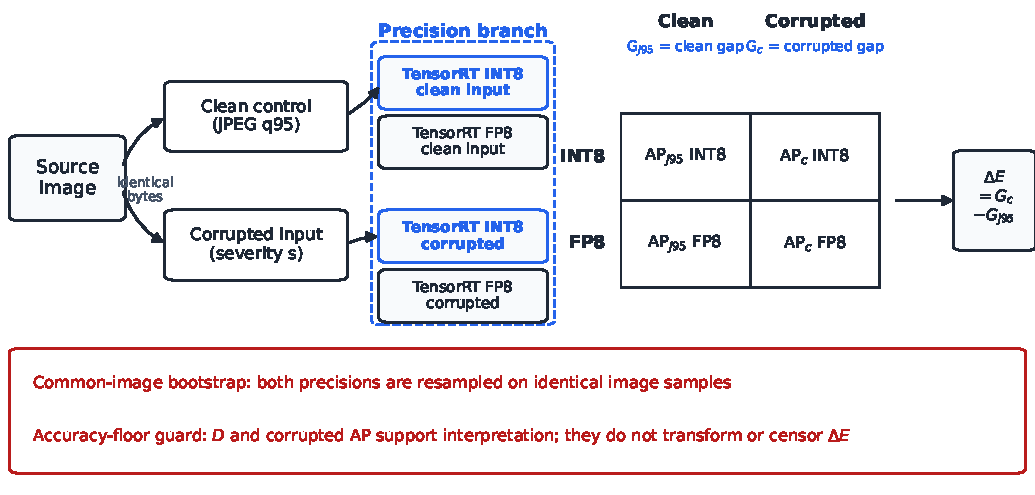
\includegraphics[width=\textwidth]{fig_framework.pdf}
\caption{Paired evaluation protocol. Each source image yields a clean control re-encoded at JPEG quality 95 ($\Jclean$) and corrupted inputs that are also re-encoded at quality 95, so the INT8 and FP8 engines receive identical bytes. The four AP cells give the clean gap $G_0$ and the corrupted gap $G_c$, and $\Delta E=G_c-G_0$. The FP32 reference cancels from $\Delta E$ and is not shown.}
\label{fig:framework}
\end{figure*}

\section{Methods}
\label{sec:methods}

\subsection{Treatments and arms}

A \emph{treatment} is the complete recorded configuration of an executable detector: checkpoint, ONNX graph, quantize/dequantize (Q/DQ) placement, calibration list and preprocessing, excluded operators, TensorRT builder settings, runtime, and decoder. ``INT8'' and ``FP8'' therefore qualify treatments, not isolated datatypes; an \emph{arm} is one treatment within an experiment. All engines were built with TensorRT 11.1.0.106~\citep{nvidia2026tensorrt} on an NVIDIA GeForce RTX 5090 from ONNX graphs quantized by NVIDIA ModelOpt with entropy calibration~\citep{nvidia2026modelopt,migacz2017entropy}; study-built registries record ModelOpt 0.45.0, and the older YOLO11 registries do not record its version.

Builder policy is recorded per engine. The YOLO11 engines predate the frozen analysis and were built by \texttt{trtexec} with TensorRT defaults (TF32 enabled). The RetinaNet quantized arms were built with the TensorRT Python builder and TF32 disabled; the older RetinaNet FP32 and legacy arms use TF32. Within each family, all quantized arms entering a $\Delta E$ contrast share one TF32 setting. Paired and intervention arms are calibrated on 512 deterministically selected training images, disjoint from the evaluation images; the diagnostic sweeps also include 128-image and max-estimator variants (Table~\ref{tab:decomposition}).

The RetinaNet arms are:
\begin{itemize}[leftmargin=1.45em,itemsep=1pt,topsep=2pt,parsep=0pt]
  \item \textbf{INT8-legacy}: the historical recipe, whose calibration preprocessing differs from inference preprocessing; retained as a diagnostic arm.
  \item \textbf{INT8-matched}: entropy INT8 with calibration preprocessing identical to inference and the same 512-image budget as FP8.
  \item \textbf{INT8-selective}: INT8-matched with all \texttt{/head/regression\_head/} nodes excluded from quantization (head convolutions run in fp16); no retraining.
  \item \textbf{INT8-corruptcalib}, \textbf{INT8-sel-corruptcalib}: matched and selective recipes calibrated on noise and JPEG corruptions (fold~1); \textbf{INT8-cc2calib}, \textbf{INT8-sel-cc2calib}: the same on fog and motion blur (fold~2; Section~\ref{sec:intervention-design}).
  \item \textbf{INT8-q95calib}, \textbf{INT8-sel-q95calib}: codec controls calibrated on the same 512 clean images re-encoded at JPEG quality 95.
  \item \textbf{FP8-matched}, \textbf{FP32}: matched-recipe FP8 and the full-precision reference. An older \textbf{FP8-legacy} engine is cited for context only.
\end{itemize}
Table~\ref{tab:glossary} defines the remaining terms.




\begin{table}[h]
\centering
\caption{Terminology.}
\label{tab:glossary}
\footnotesize
\begin{tabular}{@{}p{0.22\columnwidth}p{0.72\columnwidth}@{}}
\toprule
Term & Meaning \\
\midrule
contract-matched & calibration preprocessing identical to inference \\
codec-matched & sharing the final JPEG quality-95 encoding \\
paired & evaluated on identical images and bootstrap resamples \\

cell & one corruption$\times$severity condition (12 per evaluation) \\
$\Jclean$ control & clean image re-encoded at JPEG quality 95 \\
level deficit & AP shortfall an arm already carries on clean inputs \\
$\Delta E$ & change in an AP gap under corruption relative to the clean control \\
severity wall & a saturated cell where all arms sit near the accuracy floor \\
ledger & hash-addressed JSON record of inputs, predictions, or metrics \\
frozen / post hoc & fixed at the relevant protocol freeze / added after it \\
in-family / held-out & corruption families inside / outside a calibration fold \\
\bottomrule
\end{tabular}
\end{table}

\subsection{Paired estimand}
\label{sec:estimands}

For dataset $d$, model $m$, treatment $q$, and condition $c$, $\AP_{d,m,q,c}$ denotes COCO-style AP@[.5:.95] in AP points, and $\Jclean$ denotes the clean control, i.e., the source image encoded at JPEG quality 95 without corruption (Fig.~\ref{fig:framework}). The FP8--INT8 gaps on clean and corrupted inputs are
\begin{equation}
G_{d,m,x}=\AP_{d,m,\mathrm{FP8},x}-\AP_{d,m,\mathrm{INT8},x},
\quad x\in\{\Jclean,c\},
\end{equation}
and the primary interaction is
\begin{equation}
\Delta E_{d,m,c}=G_{d,m,c}-G_{d,m,\Jclean}.
\label{eq:delta-e}
\end{equation}
A positive $\Delta E$ indicates that the FP8--INT8 gap widens under corruption, and a negative value that it narrows; the FP32 reference cancels. With $G_0=G_{d,m,\Jclean}$ and $G_{\mathrm{corr}}$ the mean of $G_{d,m,c}$ over the 12 corruption--severity cells, the per-block estimand is $\Delta E=G_{\mathrm{corr}}-G_0$. The contrast is descriptive; it has the algebra of a difference-in-differences interaction~\citep{angrist2009mostly} without a causal claim. $\Delta E$ is scale-sensitive: if both treatments retain the same fraction $r$ of their clean AP, then $\Delta E=(r-1)G_0$, which is negative whenever $G_0>0$ and $r<1$. Every $\Delta E$ is therefore reported together with the clean gap and the absolute corrupted AP (the floor guard), so that a gap that shrinks near a shared accuracy floor is not read as robustness.

The same construction applies to two arms of one format (for example, INT8-selective minus INT8-matched), which isolates a single recipe component. Restricting the corrupted set to a subset $S$ gives the intervention contrast
\begin{equation}
\Delta E_{A-B,\,S}=\big[\AP_A-\AP_B\big]_{S}-\big[\AP_A-\AP_B\big]_{\Jclean},
\label{eq:delta-cal}
\end{equation}
denoted $\Delta E_{\text{held-out}}$ or $\Delta E_{\text{in-family}}$. For an intervention-minus-baseline contrast, a positive value is a corruption-specific benefit; for the FP8$-$INT8 order of Eq.~\eqref{eq:delta-e}, it means that the FP8 advantage grows.

Two quantities are kept separate. The \emph{level deficit} is an arm's AP shortfall to a comparator that is already present on clean inputs (equal to $G_0$ when the comparator is the paired FP8 arm). The \emph{interaction} $\Delta E$ is what corruption adds. The RetinaNet INT8-matched arm, for example, has a large level deficit but a negative $\Delta E$ on KITTI.

\subsection{Corruptions and codec control}
\label{sec:corruptions}

Four synthetic corruptions are generated deterministically at three severities (labels 1/3/5): Gaussian noise ($\sigma\in\{8,20,40\}$ on the 0--255 scale), linear motion blur (kernel lengths $\{5,13,23\}$, random angle), fog (strength--radius pairs $(0.18,6)$, $(0.38,12)$, $(0.62,20)$), and JPEG compression (qualities $\{70,40,15\}$). Every output is re-encoded at JPEG quality 95, so clean controls and corrupted inputs share the final codec, and a SHA-256-derived seed binds dataset, image, corruption, and severity. Inference uses a 640-pixel letterbox and family-specific decoders: YOLO11 uses a confidence threshold of 0.001 and class-wise NMS at an intersection-over-union (IoU) of 0.7; RetinaNet uses 0.05 and batched NMS at IoU 0.5; both keep at most 300 detections. AP follows the COCO protocol (\texttt{pycocotools}, \texttt{maxDets}=100). Decoder settings are identical within a family, so cross-family comparisons compare whole recipes.

\subsection{Datasets and checkpoints}
\label{sec:datasets}

Three evaluation sets are used: KITTI validation (1,496 images)~\citep{geiger2012kitti}, PASCAL VOC2007 test (4,952 images)~\citep{everingham2015voc}, and a fixed 2,000-image subset of COCO val2017~\citep{lin2014coco} (seed 20260924). VOC and KITTI annotations were converted from Ultralytics YOLO labels to COCO format; VOC objects marked difficult are omitted rather than kept as ignore regions, so detections on them count as false positives, and KITTI keeps eight Ultralytics categories and drops \texttt{DontCare} regions. KITTI and VOC YOLO11 models were fine-tuned from Ultralytics weights and selected by the Ultralytics best-fitness rule; RetinaNet ResNet-50-FPN-v2 models were fine-tuned for 100 epochs at 640-pixel input (seed 20260807) and selected by minimum validation loss. Both selections used the evaluation partition, so absolute KITTI and VOC AP is optimistic. COCO YOLO11 uses the official checkpoint. Each block covers original clean images, the codec control, and 12 corruption cells (14 conditions per arm; 13 for the older RetinaNet FP32 and legacy arms). All checkpoint, split, and training manifests are hash-bound (Supplement S4).

The KITTI evaluation set is the 1,496-image Ultralytics validation partition of the 7,481-image training set. All KITTI checkpoints of the paired, intervention, and post-hoc layers (YOLO11, RetinaNet, FCOS) were trained on the complementary 5,985-image partition. A later frame-level resplit (\texttt{kitti\_confirmatory\_v1}, seed 20260818) keeps the same 1,496 images for selection and divides the 5,985 images into 4,788 training and 1,197 ``final'' images; because the checkpoints above saw all 5,985 images, the final partition is not held out from them. A holdout for a retrained checkpoint was therefore obtained by training RetinaNet on the 4,788 images only (Section~\ref{sec:wa-fcos-design}). KITTI images are frames from a limited number of driving sequences, and the split is by frame, so drives appear on both sides of every partition boundary; under a 16${\times}$16 average hash, 3\% of the 512 calibration images (13/512) have an identical-hash evaluation frame and 12\% have a match within distance~5. Each image was mapped to its raw drive with the official devkit for a drive-clustered bootstrap (Section~\ref{sec:bootstrap}).


The KITTI validation set was used while the selective recipe was developed, so KITTI selective-arm estimates on it are development-contaminated; VOC, the COCO-pretrained replication (Section~\ref{sec:coco-pretrained}), and the retrained KITTI holdout are cleaner checks. RetinaNet is evaluated on KITTI and VOC only, so the frozen paired COCO evidence comes from YOLO11 alone.

\subsection{Statistical inference}
\label{sec:bootstrap}

Intervals describe uncertainty from the finite set of evaluation images, with checkpoints, engines, calibration, and corruptions fixed~\citep{bouthillier2021variance,pineau2021reproducibility}. Within each dataset$\times$model block, one deterministic schedule of 2,000 image resamples~\citep{efron1979bootstrap} is shared by all arms and conditions, so every contrast is computed on common resamples. Point estimates are full-sample values; intervals are 2.5th--97.5th bootstrap percentiles, marked \sigstar{} when they exclude zero. Two-sided $p$-values use the plus-one rule $\widetilde p=\min\{1,\,2(b_{\min}{+}1)/(B{+}1)\}$ (minimum $2/2001\approx0.001$), where $b_{\min}$ is the smaller of the numbers of draws $\le0$ and $\ge0$; the $p$-values are Holm-adjusted across the nine YOLO11 blocks~\citep{holm1979simple}. Heterogeneity across blocks is tested with Cochran's $Q$~\citep{cochran1954combination,higgins2002quantifying} and, because blocks of one dataset share images, also with a generalized $Q$ that uses the covariance from a rerun with a dataset-shared schedule. As a sensitivity analysis, KITTI intervals on the validation partition are recomputed by resampling its \nnClDrives{} drives ($B=1{,}000$; Supplement S9); the retrained holdout uses the drive mapping of the final partition (Supplement S15). Diagnostic decomposition arms are single runs without intervals.

\subsection{Corruption-aware calibration}
\label{sec:intervention-design}

\begin{figure*}[t]
\centering
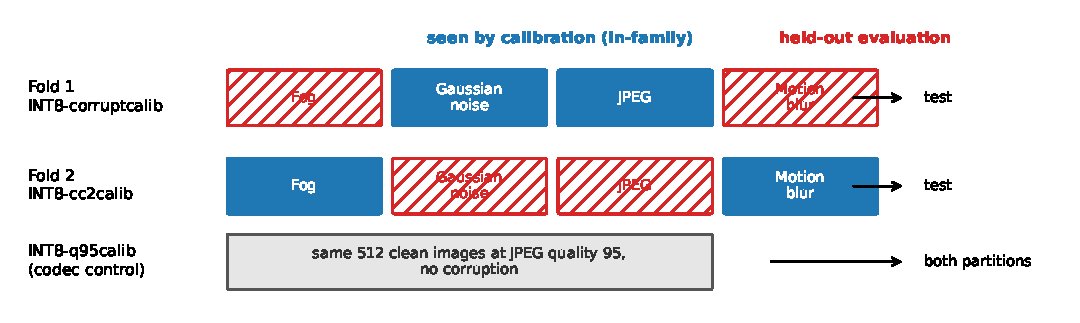
\includegraphics[width=0.92\textwidth]{nn_fold_design.pdf}
\caption{Corruption-calibration folds and the codec-matched control arm. Filled blue cells are families seen by entropy calibration (the in-family partition); hatched red cells are held out and never calibrated. Fold~1 (INT8-corruptcalib) calibrates Gaussian noise and JPEG and is tested on fog and motion blur; fold~2 (INT8-cc2calib) swaps the roles. INT8-q95calib sees only the same 512 clean images re-encoded at JPEG quality~95 and is evaluated on both partitions. Selective-tier arms (sel-corruptcalib, sel-cc2calib, sel-q95calib) share each fold's split.}
\label{fig:folds}
\end{figure*}

The intervention tests one hypothesis under decision rules frozen before any intervention run: \emph{if INT8-matched corrupted-input accuracy is limited because calibration images never show corrupted activation ranges, calibration on corrupted images should recover AP on held-out corruptions.} The hypothesis concerns corrupted-input accuracy and cannot explain the clean deficit. Each of the 512 calibration images is assigned by a hash of its path (schedule \texttt{nn-corruptcalib-v1}) to one of six in-family cells (77--102 images each) and corrupted with the evaluation parameters and JPEG-95 encoding. Fold~1 calibrates on Gaussian noise and JPEG and holds out fog and motion blur; fold~2 swaps the roles (75--95 images per cell; Fig.~\ref{fig:folds}). The full tier re-quantizes INT8-matched, and the selective tier re-quantizes INT8-selective.

\begin{table}[t]
\centering
\caption{Intervention decision rules and their registration status. ``dir.'': read directionally, so a significant harm counts as failure. ``null-seek'': met only when the interval contains zero; this bounds the residual but does not prove equivalence. \textsuperscript{a}The registered wording is two-sided (interval excluding 0 in either direction); the text uses the directional reading. \textsuperscript{b}Registered as a primary estimand, not a success criterion. The codec-matched (q95calib) controls are post hoc for fold~1 and pre-specified for fold~2.}
\label{tab:rules}
\scriptsize
\setlength{\tabcolsep}{3pt}
\begin{tabular}{@{}llll@{}}
\toprule
Contrast & Tier & Fold 1 & Fold 2 \\
\midrule
Held-out gain vs clean-calib.\ arm & full & frozen, dir. & frozen, dir.\textsuperscript{a} \\
Held-out $\Delta E$ vs matched/q95 & full & post hoc & frozen, dir. \\
Held-out gain vs clean-calib.\ arm & sel. & frozen estimand\textsuperscript{b} & post hoc \\
Held-out residual vs FP8 incl.\ 0 & sel. & frozen, null-seek & post hoc \\
\bottomrule
\end{tabular}
\end{table}

Table~\ref{tab:rules} lists the rules. Fold~1 has two success criteria: (i)~the full-tier arm improves the held-out corrupt mean over INT8-matched with an interval above zero, supporting the range-mismatch hypothesis; (ii)~the held-out mean of the selective arm is compatible with FP8-matched, which would let calibration explain the VOC residual. Criterion (ii) seeks a null and has no equivalence margin. Fold~2 was frozen before its runs and pre-specifies, for the full tier, a replication of criterion (i) and a corruption-specific rule: $\Delta E_{\text{held-out}}$ must exceed zero against both INT8-matched and INT8-q95calib. Its selective-tier contrasts are post hoc.

The fold-2 replication rule is worded two-sidedly (``CI95 excluding 0 $\Rightarrow$ fold-1 frozen criterion replicated''). It is read through the directional fold-1 criterion it cites, so a significant held-out decrease counts as failure; the literal reading would change only the KITTI verdict. In-family gains alone indicate calibration fitting, not transfer. All rules are reported regardless of outcome.

Two analyses were added after the fold-1 freeze: a comparison of held-out gains with the remaining deficit to FP8-matched, and the corruption-specific component $\Delta E_{\text{held-out}}$, which removes the shift that also appears on clean inputs. The subtraction is an arithmetic interaction on the AP scale; reading it as a corruption-specific benefit assumes that the clean effect carries over additively, and scale or floor effects can also produce a nonzero value (Supplement S8).

Corrupt-calibration images carry the JPEG-95 encoding of the evaluation images, whereas the clean calibration list uses the original files, so a gain over INT8-matched could reflect codec adaptation. The q95calib controls isolate this effect. They were added after the fold-1 results and are post hoc for fold~1 but pre-specified for fold~2. Codec adaptation can shift AP in either direction, so held-out gains are attributed to corruption coverage only if they also hold against the codec-matched anchor.

\subsection{Post-hoc analyses}
\label{sec:wa-fcos-design}

The analyses below were specified after the paired-analysis freeze, reuse the frozen conditions, and are reported regardless of outcome.

\emph{Operand factorial.} Two variants of the frozen INT8-matched graph quantize only one operand class of the regression head: INT8 weights with fp16 activations (W-only) and fp16 weights with INT8 activations (A-only). Only the head's Q/DQ edges are rewired, and each rewired edge was checked against the selective graph. With the matched and selective arms, this gives a $2{\times}2$ factorial over head weights and head activations, with interaction selective$-$W-only$-$A-only$+$matched. Rewiring acts on the consumer side, so ``head activations'' include the FPN feature maps that enter the head.

\emph{FCOS.} Anchor-free FCOS (ResNet-50-FPN)~\citep{tian2019fcos} was trained on the same KITTI and VOC partitions with the same profile and run through the same matched and selective arms; the selective exclusion also covers the centerness output, which torchvision places in the regression head. The FCOS decoder reproduces torchvision post-processing exactly on 32 synthetic head outputs (Supplement, \texttt{decoder\_validation.json}); this validates the post-processing arithmetic, not end-to-end engine parity. The VOC FCOS training loss diverged at epoch~70, long after its epoch-10 selection point.

\emph{Pretrained checkpoints.} To remove dependence on the training pipeline, the same four arms were run on torchvision's COCO-pretrained RetinaNet-R50-FPN-v2 and FCOS-R50-FPN, without fine-tuning or selection on evaluation data, on the paired COCO subset, with calibration on 512 disjoint COCO train2017 images.

\emph{Retrained KITTI holdout.} RetinaNet was retrained with the frozen profile (100 epochs, seed 20260807) on the 4,788-image resplit training list and selected on the 1,496-image selection set. All six arms (FP32, FP8-matched, INT8-matched, INT8-selective, W-only, A-only) were rebuilt with the TensorRT Python builder (TF32 disabled) and evaluated on the 1,197 final images under all 14 conditions (\texttt{nn\_kitti\_holdout\_v2\_20261002}); the five quantized arms used the frozen recipes and 512 calibration images from the training list. For the retrained checkpoint, these images were excluded from training, checkpoint selection, and calibration; the recipes themselves were developed earlier on checkpoints that had seen them, so the evaluation tests fixed recipes on images unseen by the evaluated model. They share drives with the training list, so the holdout is image-disjoint but not sequence-disjoint; intervals use the image bootstrap and, as a check, the drive-clustered bootstrap.



\emph{Range-estimator counterfactuals.} INT8-matched and INT8-selective were rebuilt with max instead of entropy calibration (Supplement~S14). In a second, more local counterfactual, the scale of every activation quantizer consumed by the regression head was set to the calibration-set maximum of its tensor, with all other scales unchanged. Five of these quantizers sit on FPN inputs shared with the classification head, so the patch is local to the regression tower but not at the shared boundary. The patch is scripted (\texttt{src/patch\_maxreg\_scales.py}; scale $=\mathrm{fp16}(|x|_{\max}/127)$) and reproduces the archived graphs exactly. Both counterfactuals are single builds reported as point estimates.

\emph{Activation and Q/DQ audits.} On each graph's 512-image calibration set, every activation tensor consumed by a regression- or classification-head node of the FP32 graph was captured and summarized by per-channel $|x|_{\max}$ and excess kurtosis, aggregated as medians by FPN level. The granularity and layout of every activation scale in the frozen INT8 graphs were also recorded.






\subsection{Evidence layers}
\label{sec:evidence-layers}

Table~\ref{tab:evidence-layers} lists the seven evidence layers and their inferential status. The freeze of the paired analysis covers the analysis plan (estimands, conditions, bootstrap schedule), not the artifacts: the YOLO11 engines and partitions were built earlier and are shared with the historical layer.

\begin{table}[t]
\centering
\caption{Evidence layers and their inferential status.}
\label{tab:evidence-layers}
\footnotesize
\setlength{\tabcolsep}{4pt}
\begin{tabular}{@{}>{\raggedright\arraybackslash}p{0.19\columnwidth}>{\raggedright\arraybackslash}p{0.43\columnwidth}>{\raggedright\arraybackslash}p{0.28\columnwidth}@{}}
\toprule
Layer & Content & Inference \\
\midrule
Diagnostic & Recipe sweeps that located the fragile region & Single runs \\
Frozen paired & Nine YOLO11 blocks; RetinaNet matched arms & Bootstrap; Holm over YOLO11 \\
Intervention & Two calibration folds with codec controls & Bootstrap, unadjusted \\
Historical & Earlier 144-cell YOLO11 grid & Context only \\
Post-hoc arms & Operand factorial, FCOS, retrained KITTI holdout & Bootstrap, unadjusted \\
Pretrained & COCO-pretrained RetinaNet and FCOS & Bootstrap, unadjusted \\
Audits & Max calibration, activations, Q/DQ, latency, rebuilds & Point estimates \\
\bottomrule
\end{tabular}
\end{table}

\section{Results}
\label{sec:results}

\begin{figure*}[t]
\centering
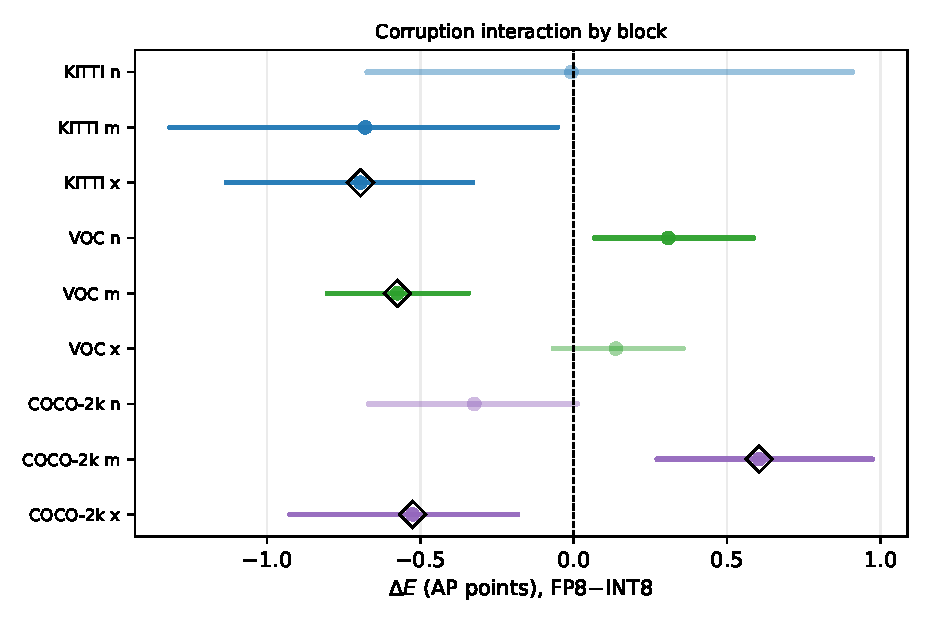
\includegraphics[width=0.72\textwidth]{nn_deltae_forest.pdf}
\caption{Paired corruption interaction $\Delta E$ (FP8$-$INT8) with 95\% common-image bootstrap intervals. Opaque markers and intervals: unadjusted interval excludes zero; faded: interval includes zero. Open diamonds: significant after Holm adjustment across the nine blocks ($p_{\mathrm{Holm}}<0.05$). The sign changes across dataset$\times$model blocks, so no single format-level effect summarizes the interaction.}
\label{fig:forest}
\end{figure*}

\subsection{YOLO11: the FP8--INT8 interaction changes sign}
\label{sec:yolo-results}

Table~\ref{tab:yolo-deltae} and Fig.~\ref{fig:forest} report the nine YOLO11 blocks. FP8 exceeds INT8 in clean-control AP in every block ($G_0$ from \nnGZeroMin{} to \nnGZeroMax{} AP) and in the 12-cell corrupt mean, although a few individual cells reverse the order. The change in this gap under corruption, however, has no stable sign: $\Delta E$ is positive on VOC/YOLO11n (\nnDEciVocN) and COCO-2k/YOLO11m (\nnDEciCocoM), negative on VOC/YOLO11m (\nnDEciVocM), KITTI/YOLO11m (\nnDEciKittiM), KITTI/YOLO11x (\nnDEciKittiX), and COCO-2k/YOLO11x (\nnDEciCocoX), and compatible with zero elsewhere (unadjusted). On VOC alone, the sign changes with model scale ($\nnDEVocN$, $\nnDEVocM$, and $\nnDEVocX$ for n, m, and x). Neither uniform INT8 fragility nor uniform equivalence is supported; with the recipe fixed, the interaction depends on dataset and model.

Cochran's test rejects a common $\Delta E$ ($Q=\nnHetQ$, $\nnHetDf$ df, $p\approx\nnHetP$; $I^2=\nnHetIsq\%$; $\tau=\nnHetTau$ AP). Accounting for the shared images within a dataset through the covariance of a shared-schedule rerun ($B=\nnHetGlsDraws$; per-draw correlations $|r|\le0.24$) leaves the result unchanged (generalized $Q=\nnHetGlsQ$, $p\approx\nnHetGlsP$). Heterogeneity also holds within VOC ($Q=\nnHetGlsQVoc$, $p\approx\nnHetGlsPVoc$) and COCO ($Q=\nnHetGlsQCoco$, $p\approx\nnHetGlsPCoco$), where only model scale varies, but not within KITTI ($Q=\nnHetGlsQKitti$, $p=\nnHetGlsPKitti$). After Holm adjustment, which requires no independence between blocks, \nnHolmSurvivors{} blocks remain significant with \emph{both} signs: COCO-2k/YOLO11m is positive, and KITTI/YOLO11x, VOC/YOLO11m, and COCO-2k/YOLO11x are negative. The DerSimonian--Laird mean of $\nnReMean$ AP (\nnReMeanCi) is only a descriptive average. Within VOC, YOLO11n and YOLO11m differ by $\nnVocNmDiff$ AP ($z=\nnVocNmZGls$ with covariance).

Heterogeneity also appears across corruption families within blocks (Fig.~\ref{fig:familyheat}); on VOC/YOLO11x, for instance, JPEG contributes $\nnFamVocXJpeg$~AP whereas Gaussian noise and motion blur contribute $\nnFamVocXGn$ and $\nnFamVocXMb$~AP. Removing the saturated motion-blur-s5 cell barely changes the heterogeneity ($Q\approx\nnHetQEx$, $I^2\approx\nnHetIsqEx\%$) and preserves the sign of every Holm-significant block; the two non-significant KITTI blocks move (YOLO11n from $\nnDEKittiN$ to $\nnDEexKittiN$; YOLO11m becomes compatible with zero; Supplement S9). Under the drive-clustered bootstrap, KITTI/YOLO11x remains negative (\nnClYoloXKitti), whereas KITTI/YOLO11m becomes compatible with zero (\nnClYoloMKitti).
The codec control behaves as intended: $\Jclean$ AP stays within \nnJCleanFid{} AP of original clean AP for every arm, and within-model retention (corrupt mean over $\Jclean$ AP) ranges from \nnRetMin{} to \nnRetMax{}, with INT8 and FP8 differing by at most \nnRetDiff.

\begin{table*}[t]
\centering
\caption{Frozen paired-analysis contrasts, FP8 minus INT8, per dataset$\times$model block. FP8/INT8 corr.\ AP: absolute 12-cell corrupt-mean AP (floor guard). $G_0$: clean-control ($\Jclean$) gap. $G_{\mathrm{corr}}$: corrupt-mean gap, computed before the absolute columns are rounded. $\Delta E=G_{\mathrm{corr}}-G_0$ with paired-bootstrap interval; \sigstar{} interval excludes zero. $p_{\mathrm{Holm}}$: two-sided bootstrap $p$-value, Holm-adjusted across the nine blocks, with the plus-one rule $\widetilde p=\min(1,\,2(b_{\min}{+}1)/(B{+}1))$ at $B{=}2000$; the smallest possible raw and adjusted values are $2/2001\approx0.001$ and $9{\times}2/2001\approx0.009$. Bold: blocks significant after Holm adjustment.}
\label{tab:yolo-deltae}
\footnotesize
{\scriptsize\setlength{\tabcolsep}{2.5pt}\begin{tabular}{llrrrrllr}
\toprule
Dataset & Model & FP8 corr.\ AP & INT8 corr.\ AP & $G_0$ & $G_{\mathrm{corr}}$ & $\Delta E$ & 95\% interval & $p_{\mathrm{Holm}}$ \\
\midrule
KITTI & YOLO11n & 44.1 & 41.9 & +2.14 & +2.13 & -0.01 & $[-0.67,\,+0.91]$ & 0.915 \\
KITTI & YOLO11m & 50.4 & 47.1 & +3.97 & +3.29 & -0.68\sigstar & $[-1.32,\,-0.05]$ & 0.128 \\
KITTI & YOLO11x & 51.0 & 50.3 & +1.44 & +0.74 & {\boldmath\bfseries -0.69\sigstar} & {\boldmath\bfseries $[-1.13,\,-0.33]$} & {\boldmath\bfseries 0.016} \\
VOC & YOLO11n & 44.8 & 43.8 & +0.68 & +0.99 & +0.31\sigstar & $[+0.07,\,+0.59]$ & 0.080 \\
VOC & YOLO11m & 51.8 & 50.7 & +1.70 & +1.12 & {\boldmath\bfseries -0.57\sigstar} & {\boldmath\bfseries $[-0.80,\,-0.34]$} & {\boldmath\bfseries 0.009} \\
VOC & YOLO11x & 54.3 & 53.3 & +0.91 & +1.05 & +0.14 & $[-0.07,\,+0.36]$ & 0.356 \\
COCO-2k & YOLO11n & 28.2 & 27.4 & +1.10 & +0.78 & -0.32 & $[-0.67,\,+0.01]$ & 0.171 \\
COCO-2k & YOLO11m & 38.0 & 36.5 & +0.89 & +1.49 & {\boldmath\bfseries +0.60\sigstar} & {\boldmath\bfseries $[+0.27,\,+0.97]$} & {\boldmath\bfseries 0.016} \\
COCO-2k & YOLO11x & 42.4 & 41.9 & +1.00 & +0.47 & {\boldmath\bfseries -0.53\sigstar} & {\boldmath\bfseries $[-0.93,\,-0.18]$} & {\boldmath\bfseries 0.024} \\
\bottomrule
\end{tabular}
}
\end{table*}

\begin{figure*}[t]
\centering
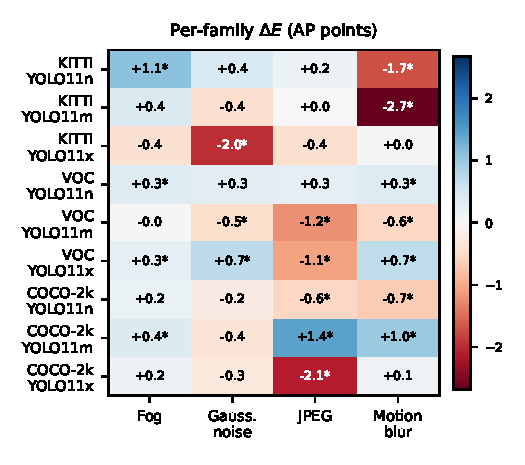
\includegraphics[width=0.5\textwidth]{nn_family_heatmap.pdf}
\caption{Per-family interaction $\Delta E$ (FP8 minus INT8, $\Jclean$ basis) for the nine paired blocks, in AP. Star: unadjusted 95\% bootstrap interval excludes zero. Every corruption family takes both signs across blocks. Two blocks have a single sign (VOC/YOLO11n positive, VOC/YOLO11m negative); the other seven mix signs, although the one positive cell of KITTI/YOLO11x is close to zero ($\nnFamKittiXMb$).}
\label{fig:familyheat}
\end{figure*}

\subsection{RetinaNet: the INT8 deficit sits in the regression head}
\label{sec:retinanet-results}

Recipe effects are much larger in RetinaNet (Table~\ref{tab:retinanet}, Fig.~\ref{fig:severity}).

\begin{figure*}[t]
\centering
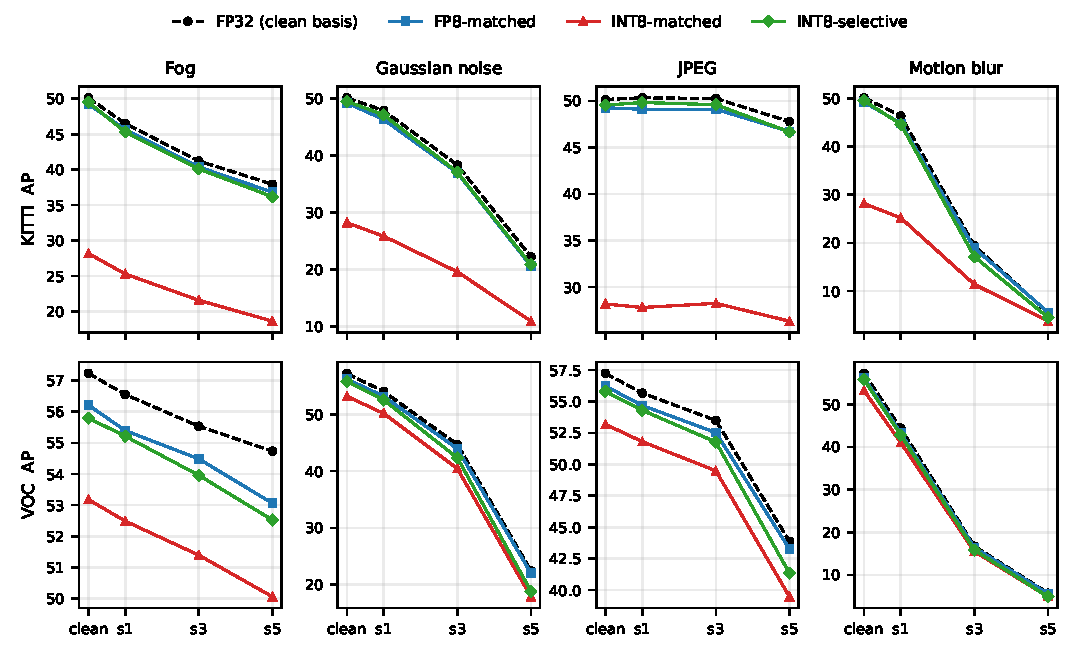
\includegraphics[width=\textwidth]{nn_retinanet_severity.pdf}
\caption{RetinaNet AP by corruption family and severity for the four matched-protocol arms on KITTI (top) and VOC (bottom). The ``clean'' point is the $\Jclean$ codec control for the matched arms and the original clean image for FP32 (dashed), which predates the codec control. INT8-matched lies far below the other arms on KITTI and somewhat below them on most VOC cells, although the VOC interaction is compatible with zero. INT8-selective tracks FP8-matched on most families; on KITTI its residual grows significantly under motion blur. All four arms collapse at motion-blur severity 5.}
\label{fig:severity}
\end{figure*}

\emph{Preprocessing mismatch.} About half of the historical INT8 collapse is caused by mismatched calibration preprocessing. In a controlled diagnostic that changes only the preprocessing (TF32 disabled, 128 calibration images), KITTI $\Jclean$ AP rises from \nnDiagLegacyJ{} to \nnDiagMatchedJ{}, recovering \nnDiagPreprocGain{} of the \nnDiagFpEightDeficitJ{}-point gap to the diagnostic FP8 build. Under the frozen protocol the historical engine scores \nnArmLegacyCleanKitti{} AP against \nnArmInCleanKitti{} for INT8-matched, but that pair also differs in TF32 setting, so the diagnostic is the cleaner attribution.

\emph{Residual deficit.} After this repair, INT8-matched still trails FP8-matched by \nnMatchedCleanDeficitKitti{} AP on KITTI but only \nnMatchedCleanDeficitVoc{} AP on VOC (original clean images; \nnMatchedGapKitti{} and \nnMatchedGapVoc{} on $\Jclean$). The interaction $\Delta E$ is \nnMatchedDEKitti{} on KITTI and \nnMatchedDEVoc{} on VOC. The KITTI narrowing follows from the scale property of $\Delta E$: INT8-matched starts about 21 AP lower and both arms retain similar fractions of their clean AP (\nnRetKittiIn{} versus \nnRetKittiFe).

\emph{Decomposition.} The diagnostic arms on KITTI place the collapse in the regression head (Table~\ref{tab:decomposition}; single runs). Quantizing only the classification head preserves accuracy (\nnDiagClsJ{}), quantizing only the regression head reproduces the collapse (\nnDiagRegJ), and quantizing everything except the regression head gives \nnDiagNoRegJ, within \nnNoRegFpGap{} AP of the diagnostic FP32 build (\nnDiagFpThirtyTwoJ). Across all eleven INT8 arms, every arm that quantizes the regression head scores \nnDiagLegacyJ{}--\nnDiagSharedMaskJ{} AP, regardless of preprocessing, estimator, budget, or placement, and every arm that does not scores \nnDiagBackboneJ{}--\nnDiagClsJ{} AP. Graph position does not explain the split, because the equally terminal classification head shows no measurable loss; nor does the number of quantized sites, because the restricted Conv+Add placement (\nnDiagConvAddJ) quantizes fewer sites than full INT8 yet does worse, whereas quantizing backbone and FPN (\nnDiagBackboneJ) does well. Quantizing both heads (\nnDiagHeadsJ) is worse than quantizing the whole graph, so the effects are not additive. These single development-set builds guided the design; the frozen protocol tests the exclusion itself.

\begin{table*}[t]
\centering
\caption{RetinaNet arms under the frozen protocol (COCO-style AP on converted annotations). Corrupt mean: equal weight over the 12 corruption--severity cells. $\Jclean$: codec-control clean; the FP32 and legacy arms predate the codec control (dashes). INT8-legacy is the older historical engine and also differs from the matched arms in builder policy (TF32 enabled by default versus disabled); Table~\ref{tab:decomposition} gives the controlled preprocessing-only comparison. Bold: the matched arm and its selective repair.}
\label{tab:retinanet}
\footnotesize
{\setlength{\tabcolsep}{4pt}\begin{tabular}{llrrr}
\toprule
Dataset & Arm & Clean AP & $\Jclean$ AP & Corrupt mean AP \\
\midrule
KITTI & FP32 reference & 50.15 & -- & 37.80 \\
 & FP8-matched & 49.48 & 49.25 & 36.75 \\
 & INT8-legacy (contract mismatch) & 7.21 & -- & 7.43 \\
 & INT8-matched & 28.29 & 28.18 & 20.37 \\
 & INT8-q95calib (codec control) & 28.26 & 27.85 & 20.42 \\
 & INT8-selective (reg-head FP32) & 49.60 & 49.53 & 36.58 \\
 & INT8-sel-q95calib & 50.28 & 49.79 & 36.94 \\
 & INT8-corruptcalib & 29.69 & 29.74 & 21.71 \\
 & INT8-sel-corruptcalib & 49.55 & 49.03 & 36.08 \\
 & INT8-cc2calib (fold 2) & 25.36 & 25.47 & 18.68 \\
 & INT8-sel-cc2calib (fold 2) & 49.72 & 50.54 & 37.20 \\
\midrule
VOC & FP32 reference & 57.23 & -- & 42.32 \\
 & FP8-matched & 56.17 & 56.21 & 41.48 \\
 & INT8-legacy (contract mismatch) & 33.61 & -- & 24.32 \\
 & INT8-matched & 53.30 & 53.18 & 38.71 \\
 & INT8-q95calib (codec control) & 53.33 & 53.39 & 38.54 \\
 & INT8-selective (reg-head FP32) & 55.87 & 55.79 & 40.52 \\
 & INT8-sel-q95calib & 55.81 & 55.95 & 40.40 \\
 & INT8-corruptcalib & 53.78 & 53.91 & 39.35 \\
 & INT8-sel-corruptcalib & 56.36 & 56.43 & 41.13 \\
 & INT8-cc2calib (fold 2) & 54.15 & 54.22 & 39.97 \\
 & INT8-sel-cc2calib (fold 2) & 56.40 & 56.43 & 41.58 \\
\bottomrule
\end{tabular}
}
\end{table*}

\begin{table}[t]
\centering
\caption{Diagnostic recipe decomposition on KITTI (single runs; $\Jclean$ AP; 512 calibration images unless stated). Every arm that quantizes the regression head collapses, and every arm that does not stays near FP32. The ``Matched preprocessing, 512 img'' row uses the same graph as the paired INT8-matched arm. Bold: the two arms that isolate the regression head.}
\label{tab:decomposition}
\footnotesize
{\setlength{\tabcolsep}{4pt}\begin{tabular}{lcr}
\toprule
INT8 arm & Reg.\ head INT8 & $\Jclean$ AP \\
\midrule
Legacy preprocessing, 128 img & yes & 6.72 \\
Matched preprocessing, 128 img & yes & 27.91 \\
Matched preprocessing, 512 img & yes & 28.18 \\
Max estimator, 128 img & yes & 23.94 \\
Conv+Add sites only, 128 img & yes & 15.75 \\
FP8 compute sites (shared mask) & yes & 28.74 \\
Both heads only & yes & 17.09 \\
\textbf{Regression head only} & yes & \textbf{16.41} \\
\addlinespace[2pt]
Classification head only & no & 50.57 \\
Backbone + FPN only & no & 49.14 \\
\textbf{All except regression head} & no & \textbf{49.50} \\
\addlinespace[2pt]
FP8 matched, 128 img (reference) & -- & 48.50 \\
FP32 (reference) & -- & 50.44 \\
\bottomrule
\end{tabular}
}
\end{table}


\emph{Selective repair.} Under the frozen protocol, INT8-selective is compatible with FP8-matched on KITTI for both the clean control (\nnSelResJKitti{}, FP8 minus selective) and the corrupt mean (\nnSelResCKitti{}); the clean interval spans more than one AP point, so this bounds the difference without proving equivalence. Relative to the clean gap, the residual widens under motion blur (\nnSelFamMbKitti{}) and is compatible with zero under JPEG (\nnSelFamJpegKitti{}). On VOC a small residual remains (\nnSelResJVoc{} clean, \nnSelResCVoc{} corrupt mean; $\Delta E$ \nnSelResDEVoc{}), so the regression head is the dominant but not the only source of the deficit there.

\begin{figure*}[t]
\centering
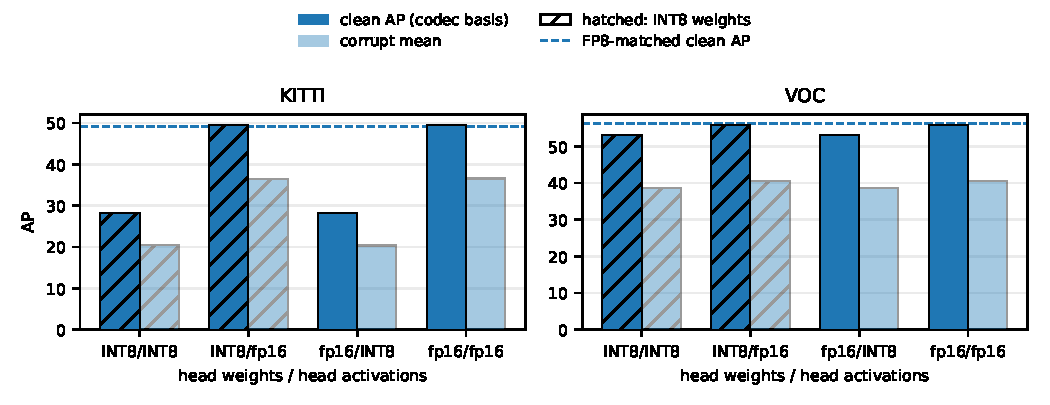
\includegraphics[width=\textwidth]{nn_wa_factorial.pdf}
\caption{Operand factorial inside the RetinaNet regression head (post-hoc arms, frozen paired conditions). Head weights and head activations are set to INT8 or fp16 independently. Solid bars: codec-control clean AP; translucent bars: 12-cell corrupt mean. With INT8 weights and fp16 activations, AP matches the selective arm within 0.1 on both datasets; with fp16 weights and INT8 activations, it matches the fully quantized arm. The deficit follows activation quantization, and the weight effect is at most about 0.2 AP (KITTI).}
\label{fig:wa-factorial}
\end{figure*}

\begin{table*}[t]
\centering
\caption{Operand decomposition of the regression-head exclusion (post-hoc arms; 95\% paired-bootstrap intervals on the $\Jclean$ basis relative to the INT8/INT8 matched arm). ``$\Jclean$ vs W8A8'': clean-level contrast to the matched arm. Unquantized operands run in fp16. Retention: corrupt-mean AP over $\Jclean$ AP. \sigstar{}: unadjusted 95\% interval excludes zero. Bold: the W-only and A-only contrasts that separate the two operands.}
\label{tab:wa-factorial}
\scriptsize
\setlength{\tabcolsep}{3pt}
{\setlength{\tabcolsep}{2.5pt}\begin{tabular}{lllllll}
\toprule
Dataset & Head weights & Head acts. & $\Jclean$ & Corrupt mean & Retention & $\Jclean$ vs W8A8 \\
\midrule
KITTI & INT8 & INT8 & 28.18 & 20.37 & 0.72 & -- \\
 & INT8 & fp16 & 49.44 & 36.52 & 0.74 & {\boldmath\bfseries $+21.25$\sigstar $[+19.88,\,+22.69]$} \\
 & fp16 & INT8 & 28.14 & 20.36 & 0.72 & {\boldmath\bfseries $-0.04$ $[-0.20,\,+0.11]$} \\
 & fp16 & fp16 & 49.53 & 36.58 & 0.74 & $+21.35$\sigstar $[+19.95,\,+22.81]$ \\
\addlinespace[4pt]
VOC & INT8 & INT8 & 53.18 & 38.71 & 0.73 & -- \\
 & INT8 & fp16 & 55.88 & 40.53 & 0.73 & {\boldmath\bfseries $+2.70$\sigstar $[+2.46,\,+2.96]$} \\
 & fp16 & INT8 & 53.19 & 38.68 & 0.73 & {\boldmath\bfseries $+0.01$ $[-0.08,\,+0.10]$} \\
 & fp16 & fp16 & 55.79 & 40.52 & 0.73 & $+2.61$\sigstar $[+2.37,\,+2.88]$ \\
\bottomrule
\end{tabular}
}
\end{table*}

\emph{Operand factorial.} The factorial (Fig.~\ref{fig:wa-factorial}, Table~\ref{tab:wa-factorial}) attributes the deficit to activation quantization. Restoring only the head \emph{activations} to fp16 raises $\Jclean$ AP to \nnWaWoJKitti{} on KITTI and \nnWaWoJVoc{} on VOC, recovering \nnWaWoSelGapKitti\% and \nnWaWoSelGapVoc\% of the selective gain; the remaining difference to full exclusion is below 0.2 AP (\nnWaSelWoJdiffKitti{} on KITTI, \nnWaSelWoJdiffVoc{} on VOC). Restoring only the head \emph{weights} leaves contrasts compatible with zero (A-only minus matched: \nnWaAoJdiffKitti{} on KITTI, \nnWaAoJdiffVoc{} on VOC; $\Delta E$ \nnWaAoDEKitti{} and \nnWaAoDEVoc{}). INT8 head weights thus cost at most about 0.2 AP; both weight-contrast point estimates are within 0.1 AP of zero, although the KITTI selective-minus-W-only interval just excludes zero. The interaction is compatible with zero on clean inputs (\nnWaIxJKitti{} on KITTI, \nnWaIxJVoc{} on VOC) and small under corruption (\nnWaIxCKitti{} on KITTI, excluding zero before adjustment; \nnWaIxCVoc{} on VOC). The much smaller FP8 loss is consistent with greater tolerance of heavy activation tails in E4M3; whether clipping or grid resolution is responsible is examined in Section~\ref{sec:discussion}.

\emph{Retrained holdout.} The pattern replicates on the 1,197 KITTI images that the retrained checkpoint never saw (Supplement~S15). INT8-matched trails FP8-matched by \nnHvFinFmInJ{} AP on $\Jclean$ inputs (\nnHvFinInJ{} versus \nnHvFinFeJ{}). This gap is smaller than for the original checkpoint, although the evaluation partition and calibration list also differ. Excluding the regression head recovers \nnHvFinSelInJ{} AP, leaving FP8 minus selective at \nnHvFinFeSelJ{}. Restoring only the head activations recovers the same amount (W-only minus matched \nnHvFinWoInJ{}), whereas restoring only the head weights does not (A-only minus matched \nnHvFinAoInJ{}). The deficit and its repair also hold under the drive-clustered bootstrap (\nnHvDrvFmInJ{} and \nnHvDrvSelInJ{}). Absolute AP on these unseen images is slightly below that on the selection set (\nnHvFinFeJ{} versus \nnHvValFeJ{} for FP8-matched).

\emph{Severity wall.} At motion-blur severity 5 every matched-protocol arm, FP32 included, falls below 6 AP on both datasets (KITTI: FP32 $\nnWallFpKitti$, FP8-matched $\nnWallFeKitti$, INT8-matched $\nnWallInKitti$, selective $\nnWallSelKitti$; VOC: $\nnWallFpVoc$, $\nnWallFeVoc$, $\nnWallInVoc$, $\nnWallSelVoc$). This shared failure compresses absolute AP gaps in that cell, and its effect on $\Delta E$ also depends on the clean gap; removing it changes no frozen-criterion verdict (Supplement~S9).


\subsection{FCOS: no head-specific deficit}
\label{sec:fcos-check}

On anchor-free FCOS~\citep{tian2019fcos} the INT8-matched arm shows no deficit of the RetinaNet kind (Table~\ref{tab:fcos}; unadjusted intervals): $\Jclean$ AP is \nnFcosArmInJKitti{} on KITTI and \nnFcosArmInJVoc{} on VOC, against \nnFcosArmFpJKitti{} and \nnFcosArmFpJVoc{} for FP32. Small FP32-minus-selective gaps remain on VOC clean inputs (\nnFcosFpJVoc) and on both corrupt means (\nnFcosFpCKitti{}, \nnFcosFpCVoc), but they are smaller than the gap of FP8-matched to FP32 and do not come from the head: excluding the regression head changes nothing measurable (selective minus matched \nnFcosSmJKitti{} and \nnFcosSmJVoc{}). INT8 even does slightly better than FP8 (FP8$-$INT8 clean \nnFcosFmJKitti{} on KITTI and \nnFcosFmJVoc{} on VOC; corrupt mean \nnFcosFmCKitti{} and \nnFcosFmCVoc{}), and the interaction is compatible with zero (\nnFcosFmDEKitti{}, \nnFcosFmDEVoc{}), although on VOC the JPEG and motion-blur family intervals exclude zero.

The RetinaNet fragility therefore does not carry over to a head that regresses per-pixel distances and a centerness score instead of anchor offsets. Because FCOS also differs in anchor density and centerness scoring, and its selective arm additionally leaves centerness unquantized, this result supports recipe dependence rather than a claim about anchor-based heads in general. The original RetinaNet and FCOS checkpoints were selected early (epochs 21 and 5 for RetinaNet on KITTI and VOC, 14 and 10 for FCOS, out of 100), but training states are not matched across families, which remains a possible explanation.

\begin{table*}[t]
\centering
\caption{Cross-architecture check (post-hoc arms): the RetinaNet regression-head deficit does not appear on FCOS. Paired-bootstrap contrasts at 95\% under the frozen conditions. On FCOS the selective-minus-matched $\Jclean$ contrast includes zero on both datasets, so no measurable head-specific INT8 cost is detected under this protocol. Each detector is a separate bootstrap block; no cross-detector contrast is estimated. \sigstar{}: unadjusted 95\% interval excludes zero. Bold: the head-exclusion effect (selective minus INT8-matched).}
\label{tab:fcos}
\scriptsize
\setlength{\tabcolsep}{3pt}
{\setlength{\tabcolsep}{2.5pt}\begin{tabular}{lllllll}
\toprule
Detector & Dataset & FP8$-$INT8 $\Jclean$ & FP8$-$INT8 $\Delta E$ & Sel$-$INT8 $\Jclean$ & Sel$-$INT8 $\Delta E$ & FP8$-$Sel $\Jclean$ \\
\midrule
RetinaNet & KITTI & $+21.07$\sigstar $[+19.57,\,+22.61]$ & $-4.69$\sigstar $[-5.49,\,-3.86]$ & $+21.35$\sigstar $[+19.95,\,+22.81]$ & $-5.14$\sigstar $[-5.94,\,-4.34]$ & $-0.28$ $[-1.11,\,+0.56]$ \\
FCOS & KITTI & $-0.47$\sigstar $[-0.990,\,-0.001]$ & $-0.04$ $[-0.44,\,+0.40]$ & $+0.00$ $[-0.15,\,+0.12]$ & $+0.00$ $[-0.13,\,+0.15]$ & $-0.47$ $[-0.99,\,+0.05]$ \\
\addlinespace[3pt]
RetinaNet & VOC & $+3.03$\sigstar $[+2.66,\,+3.41]$ & $-0.26$ $[-0.58,\,+0.06]$ & $+2.61$\sigstar $[+2.37,\,+2.88]$ & $-0.80$\sigstar $[-0.98,\,-0.61]$ & $+0.42$\sigstar $[+0.13,\,+0.74]$ \\
FCOS & VOC & $-0.14$ $[-0.33,\,+0.07]$ & $+0.07$ $[-0.13,\,+0.25]$ & $+0.01$ $[-0.04,\,+0.08]$ & $-0.03$ $[-0.09,\,+0.03]$ & $-0.16$ $[-0.36,\,+0.05]$ \\
\bottomrule
\end{tabular}
}
\end{table*}

\subsection{Replication on pretrained COCO checkpoints}
\label{sec:coco-pretrained}

Because the RetinaNet and FCOS checkpoints above share one training pipeline, the four arms were repeated on torchvision's COCO-pretrained RetinaNet-R50-FPN-v2~\citep{torchvision2026retinanet} and FCOS-R50-FPN~\citep{torchvision2026fcos} (Table~\ref{tab:coco-pretrained}).

\begin{table}[t]
\centering
\caption{Replication on pretrained checkpoints, COCO val2017 (paired 2,000-image subset; 95\% paired-bootstrap intervals, unadjusted). Arm rows give $\Jclean$ clean AP and corrupt-mean AP. Contrast rows give the difference on the $\Jclean$ basis (column~3) and the interaction $\Delta E$ (column~4). RetinaNet reproduces the head-localized INT8 deficit and its selective repair; FCOS shows no measurable head-specific cost, as in Section~\ref{sec:fcos-check}. \sigstar{}: interval excludes zero.}
\label{tab:coco-pretrained}
\scriptsize
\setlength{\tabcolsep}{2pt}
\begin{tabular}{llll}
\toprule
Detector & Arm / contrast & $\Jclean$-basis AP & Corrupt-mean / $\Delta E$ \\
\midrule
RetinaNet & FP32 & 38.30 & 31.18 \\
 & FP8-matched & 37.84 & 30.58 \\
 & INT8-matched & 34.70 & 27.97 \\
 & INT8-selective & 37.27 & 29.91 \\
\cmidrule(lr){2-4}
 & \emph{FP8$-$INT8} & $+3.14$\sigstar $[+2.78,\,+3.57]$ & $-0.53$\sigstar $[-0.90,\,-0.14]$ \\
 & \emph{Sel$-$INT8} & $+2.58$\sigstar $[+2.33,\,+2.85]$ & $-0.64$\sigstar $[-0.84,\,-0.42]$ \\
 & \emph{FP8$-$Sel} & $+0.56$\sigstar $[+0.22,\,+0.96]$ & $+0.11$ $[-0.28,\,+0.48]$ \\
\addlinespace[4pt]
FCOS & FP32 & 34.32 & 27.61 \\
 & FP8-matched & 34.24 & 27.51 \\
 & INT8-matched & 34.19 & 27.44 \\
 & INT8-selective & 34.20 & 27.45 \\
\cmidrule(lr){2-4}
 & \emph{FP8$-$INT8} & $+0.05$ $[-0.22,\,+0.27]$ & $+0.02$ $[-0.20,\,+0.28]$ \\
 & \emph{Sel$-$INT8} & $+0.01$ $[-0.06,\,+0.09]$ & $0.00$ $[-0.07,\,+0.07]$ \\
 & \emph{FP8$-$Sel} & $+0.04$ $[-0.21,\,+0.24]$ & $+0.02$ $[-0.19,\,+0.27]$ \\
\bottomrule
\end{tabular}

\end{table}

The pattern replicates. On pretrained RetinaNet, INT8-matched trails FP32 by \nnCpFmHJPRet{}~AP (FP32 \nnCpArmFpJRet, INT8 \nnCpArmInJRet, FP8-matched \nnCpArmFeJRet; FP8$-$INT8 \nnCpFmJRet). Excluding the regression head recovers about \nnCpRecovRet{}\% of the clean FP8--INT8 gap (selective minus INT8 \nnCpSmJRet; FP8 minus selective \nnCpFsJRet), the same localization at a smaller scale. On pretrained FCOS the clean FP8$-$INT8 and selective-minus-INT8 contrasts are compatible with zero (\nnCpFmJFco; \nnCpSmJFco), although small corrupt-mean deficits relative to FP32 remain. On COCO the interaction is small relative to the level gap: $\Delta E$ is \nnCpFmDERet~AP for RetinaNet, a slight narrowing, and \nnCpFmDEFco~AP for FCOS. The deficit is therefore mainly a level shift that corruption does not amplify, which limits how far the interaction framing extends beyond KITTI and VOC.

\subsection{Corruption-aware calibration}
\label{sec:intervention-results}

Table~\ref{tab:intervention-summary} summarizes the intervention on two bases: the raw held-out AP change and the corruption-specific component $\Delta E_{\text{held-out}}$ (Eq.~\eqref{eq:delta-cal}). Supplement~S7 gives all contrasts.

\begin{table*}[t]
\centering
\caption{Intervention outcome per fold$\times$dataset cell, full tier
(corrupt-calibration arm minus INT8-matched; AP with 95\% paired
intervals, unadjusted). ``Held-out change'' is the raw AP change on the
held-out families; $\Delta E_{\text{held-out}}$ subtracts the clean-control
shift and is the corruption-specific component. Verdicts use the
directional reading of Section~\ref{sec:intervention-design}; under the literal
two-sided fold-2 wording, KITTI fold~2 would also register as a detected change.}
\label{tab:intervention-summary}
\footnotesize
\begin{tabular}{@{}llll@{}}
\toprule
Cell & Held-out change & $\Delta E_{\text{held-out}}$ & Frozen verdict (directional) \\
\midrule
KITTI fold~1 & \nnCcHKitti{} & \nnCcDHKitti{} & primary met \\
VOC fold~1 & \nnCcHVoc{} & \nnCcDHVoc{} & null \\
KITTI fold~2 & \nnCtHKitti{} & \nnCtDHKitti{} & harm (fails) \\
VOC fold~2 & \nnCtHVoc{} & \nnCtDHVoc{} & met + corruption-specific \\
\bottomrule
\end{tabular}
\end{table*}

On the raw basis, the primary criterion is met on KITTI fold~1 and VOC fold~2 and is null on VOC fold~1. On KITTI fold~2, raw AP drops significantly relative to INT8-matched and INT8-q95calib, including on the calibrated families, so the criterion fails. In fold~1 the null-seeking selective criterion fails on both datasets (held-out residual to FP8-matched \nnSccFHVoc{} on VOC and \nnSccFHKitti{} on KITTI); the analogous post-hoc fold-2 contrast includes zero on VOC (\nnSctFHVoc{}) and excludes it favorably on KITTI (\nnSctFHKitti{}). Where the criterion is met, the gain is small: on KITTI fold~1 it closes less than a tenth of the gap to FP8-matched (\nnCcFHKitti{} remains). Removing the motion-blur-s5 cell changes no verdict (held-out \nnCcHxKitti{} on KITTI, \nnCcHxVoc{} on VOC).

On the interaction basis, only VOC fold~2 shows a significantly positive corruption-specific component (\nnCtDHVoc{}; \nnCtQDHVoc{} against the codec anchor). VOC fold~1 is significantly negative (\nnCcDHVoc{}), and both KITTI cells are compatible with zero. In the selective tier, fold~2 raises the KITTI held-out mean (\nnSctHKitti{}), but not against its codec anchor (\nnSctQHKitti{}), whereas the VOC fold-2 gain holds (\nnSctHVoc{}; codec-anchored \nnSctQHVoc{}). In a retention-scaled check (Supplement~S7), observed and predicted held-out changes are close in both KITTI folds (\nnCcHKittiP{} versus \nnPredCcHoKitti{}; \nnCtHKittiP{} versus \nnPredCtHoKitti{}), whereas VOC fold~2 clearly exceeds its prediction (\nnCtHVocP{} versus \nnPredCtHoVoc{}).

In the full tier, calibration on JPEG-95 images alone produces no detected change in clean AP (\nnQqJKitti{} on KITTI, \nnQqJVoc{} on VOC) and no corrupt-mean improvement; its level effects stay below 0.5 AP, but its interaction effects are as large as the corruption-specific components, so the codec-anchored contrasts decide the verdicts.

Corruption-aware entropy calibration is therefore context-dependent: one cell shows a significant corruption-specific benefit, KITTI fold~2 shows a significant raw-AP harm, and the other effects are null or negative. Neither fold repairs the KITTI level deficit. Because only the calibration images are varied, range mismatch as such is not ruled out; the change that does remove the level deficit is regression-head exclusion.

\subsection{Historical exploratory evidence}
\label{sec:historical}

An earlier 144-cell exploratory analysis of the same YOLO11 engines and estimand covered four datasets (including TT100K~\citep{zhu2016tt100k}), the full COCO codec-control pool, and additional arms, without the Holm family. It found an overall interaction of $-0.02$ AP $[-0.24,+0.15]$, $-0.55$ $[-0.78,-0.29]$ on post-selection VOC/KITTI holdouts with independently selected checkpoints, and 56 point-estimate sign disagreements between the raw corrupted-input gap and $\Delta E$, with 17 $\Delta E$ intervals entirely below zero. These results motivated the frozen analysis and are not pooled with it. Two exploratory transfer cases, RT-DETR-L~\citep{zhao2024rtdetr,carion2020detr} and legacy RetinaNet, failed in INT8 under the unmigrated recipe; a corrected recipe was not tested for RT-DETR-L.

\section{Discussion}
\label{sec:discussion}

\subsection{Recipe, not format}

All evidence layers point to one conclusion: the corruption robustness of a quantized detector depends on the recipe, the model region, and the evaluation context, not only on the format. The paired layer shows that the interaction has no stable sign, the diagnostic layer shows where the level deficit sits, and the intervention shows that the obvious remedy is itself context-dependent. On KITTI, matching calibration preprocessing raises diagnostic $\Jclean$ AP by \nnDiagPreprocGain{} points, and regression-head exclusion raises paired $\Jclean$ AP by \nnSelGainJKitti{} points; both changes are several times larger than the FP8-matched--INT8-matched corrupt-mean interaction ($\nnMatchedDEKittiP$ AP). Larger interactions occur only between arms that also differ in recipe (up to $\nnCtFDIKittiP$ AP, mostly a scale effect) or at the level of single families ($\nnMatchedFamMbKitti$ AP for KITTI motion blur). Comparing ``INT8'' and ``FP8'' robustness without the recipe can therefore reverse conclusions.

\subsection{Mechanism of the regression-head deficit}

\begin{table}[t]
\centering
\caption{AP by IoU threshold and object size, RetinaNet, $\Jclean$ basis (single runs). W-only: INT8 head weights, fp16 head activations; A-only: the reverse. Bold: AP$_{75}$ and AP$_S$ of the arms with INT8 head activations, where the deficit concentrates.}
\label{tab:iou-size}
\footnotesize
{\setlength{\tabcolsep}{3.5pt}\begin{tabular}{llrrrrrr}
\toprule
Dataset & Arm & AP & AP$_{50}$ & AP$_{75}$ & AP$_S$ & AP$_M$ & AP$_L$ \\
\midrule
KITTI & FP8-matched & 49.2 & 77.7 & 52.8 & 34.0 & 48.6 & 61.3 \\
 & INT8-matched & 28.2 & 60.3 & \textbf{21.6} & \textbf{3.0} & 23.2 & 55.4 \\
 & INT8-selective & 49.5 & 77.8 & 52.9 & 35.7 & 48.7 & 61.7 \\
 & W-only & 49.4 & 78.0 & 52.7 & 35.5 & 48.6 & 61.6 \\
 & A-only & 28.1 & 60.7 & \textbf{21.6} & \textbf{3.3} & 23.2 & 55.4 \\
\addlinespace[4pt]
VOC & FP8-matched & 56.2 & 81.0 & 60.9 & 23.6 & 37.7 & 62.2 \\
 & INT8-matched & 53.2 & 80.2 & \textbf{56.9} & \textbf{17.9} & 33.8 & 60.3 \\
 & INT8-selective & 55.8 & 80.8 & 60.5 & 23.7 & 38.2 & 61.5 \\
 & W-only & 55.9 & 80.9 & 60.7 & 23.6 & 38.3 & 61.6 \\
 & A-only & 53.2 & 80.2 & \textbf{56.9} & \textbf{17.8} & 33.7 & 60.3 \\
\bottomrule
\end{tabular}
}
\end{table}


The decomposition and the paired selective arm agree that the regression head carries the deficit, in line with detector PTQ work on regression branches~\citep{ding2024regptq}. An obvious explanation is RetinaNet's anchor-offset decoding: width and height offsets pass through an exponential, so a fixed error on the raw output becomes a proportional box error that high-IoU AP penalizes, whereas classification scores pass through a saturating sigmoid. A fixed log-scale perturbation gives a size-independent relative error, but size-stratified AP also depends on baseline localization, so the size profile of the deficit (Table~\ref{tab:iou-size}) cannot by itself separate decoding sensitivity from activation quantization. On KITTI the INT8-matched gap to FP8 is \nnIouGapSeventyFiveKitti{} AP at $\mathrm{AP}_{75}$ against \nnIouGapFiftyKitti{} AP at $\mathrm{AP}_{50}$, and $\mathrm{AP}_S$ falls to \nnIouApSmallInKitti{} against \nnIouApSmallFeKitti{}, while $\mathrm{AP}_L$ drops by only \nnIouGapLargeKitti{} AP. A-only reproduces this profile and W-only does not.

The activation captures and the Q/DQ structure refine this picture (Supplement~S13). Each FPN level has its own per-tensor activation scale at the regression head (25 head-consumed quantizers: five on the shared FPN inputs and four tower tensors at each of the five levels), so the deficit is not caused by one range shared across levels. The tails, however, are heaviest at the finest levels: median excess kurtosis is \nnActRegKurtPThreeKitti{} and \nnActRegKurtPFourKitti{} at P3 and P4 against \nnActRegKurtPSevenKitti{} at P7 on KITTI, compared with \nnActClsKurtPThreeKitti{} and \nnActClsKurtPFourKitti{} for the classification head, with the same ordering on VOC; on the pretrained COCO graph the peak is at P4 (\nnActRegKurtPFourCoco{} versus \nnActRegKurtPThreeCoco{} at P3), still well above the coarse levels (Table~S9). Heavier fine-level tails are consistent with coarser INT8 resolution near the center of the distribution at the levels that predict small objects, which would match the $\mathrm{AP}_S$ and $\mathrm{AP}_{75}$ collapse. Median per-channel maxima are similar for the two heads (\nnActRegAmaxMedKitti{} versus \nnActClsAmaxMedKitti), whereas the calibrated per-tensor ranges differ (median amax \nnActStaticRegMedKitti{} versus \nnActStaticClsMedKitti{} on KITTI); how much of the deployed range is spent on outliers was not measured. This is a distributional argument, not a causal test.

Calibration with corrupted images neither repairs the KITTI head nor yields a corruption-specific benefit there, so the results suggest a sensitivity to quantization error that none of the tested calibration sets fixes.

The range-estimator counterfactuals test the estimator directly. Graph-wide max calibration covers the full calibration range yet deepens the KITTI deficit (\nnMcMaxJKitti{} versus \nnArmInCleanKitti{} AP), while head exclusion still helps (\nnMcSelGainJKitti{} AP); on VOC it destroys the classifier's score distribution (Supplement~S14). Restricting max calibration to quantizers consumed by the regression head keeps VOC functional and still does not repair the deficit (\nnMcMaxRegJKitti{} and \nnMcMaxRegJVoc{} AP versus \nnArmInCleanKitti{} and \nnArmInCleanVoc{}). The head sensitivity is therefore not an artifact of entropy calibration, and the results favor coarse grid resolution over calibration-set clipping. Because max calibration changes clipping and resolution together, the two mechanisms are not isolated, and neither evaluation-time clipping nor rounding bias is excluded.

FP8, whose exponent field provides a wide dynamic range, quantizes the same head without failing (\nnArmFeLegacyCleanKitti{} AP for FP8-legacy and \nnArmFeCleanKitti{} AP for FP8-matched on KITTI), which also fits a dynamic-range account. FCOS fits a head-design account: its regression head predicts linearly decoded distances and shows no head-specific deficit. This support is weak, because FCOS also differs in anchor density and centerness, and the exponential decode runs after the engine, downstream of the activations implicated by the factorial.

FCOS regression-head kurtosis at P3 and P4 (\nnActRegKurtPThreeFcosKitti{} and \nnActRegKurtPFourFcosKitti{} on KITTI; \nnActRegKurtPThreeFcosVoc{} and \nnActRegKurtPFourFcosVoc{} on VOC) is far below the RetinaNet values (\nnActRegKurtPThreeKitti{} and \nnActRegKurtPFourKitti{}; \nnActRegKurtPThreeVoc{} and \nnActRegKurtPFourVoc{}); the tails are lighter but not absent. Why head exclusion helps about eight times more on KITTI than on VOC (\nnSelGainJKitti{} versus \nnSelGainJVoc{} AP) remains open; differences in object-size distributions between the datasets are one candidate.

\subsection{Practical guidance}

Four practical rules follow. (i)~Calibration preprocessing should match inference byte for byte before any quantization gap is interpreted. (ii)~Regression and classification heads should be evaluated as separate quantization regions, as in sensitivity-based mixed precision~\citep{dong2019hawq,huang2025hessianmp}; head exclusion recovered \nnSelGainJKitti{} AP on KITTI RetinaNet but nothing measurable on FCOS (\nnFcosSmJKitti{}, \nnFcosSmJVoc{}). (iii)~Corruption-augmented calibration should not be expected to transfer; its held-out effect ranged from a significant harm to a $\nnCtHVocP$-AP gain, and calibration images should share the deployment codec before gains are credited to corruption coverage. (iv)~Paired interactions should be reported with absolute corrupted AP and the clean gap.

Selective precision is the retraining-free option to try first: its contrasts with FP8-matched were compatible with zero on KITTI, without establishing equivalence, and it trailed FP8-matched by $\nnSelResJVocP$ AP (clean) and $\nnSelResCVocP$ AP (corrupt mean) on VOC. On one idle host (Supplement~S12), it is \nnLatSelOverheadMin--\nnLatSelOverheadMax\% slower than INT8-matched (\nnLatIntEightMin--\nnLatIntEightMax~ms per image) and \nnLatSelVsFpEightMin--\nnLatSelVsFpEightMax\% faster than FP8-matched (\nnLatFpEightMin--\nnLatFpEightMax~ms); FP32 references take \nnLatFpMin--\nnLatFpMax~ms. The regression head accounts for \nnRegHeadMac\% of convolution MACs; kernel-level execution precision and rates were not measured. Five rebuilds of each of seven RetinaNet arms (\nnRbTotal{} builds) gave bit-different engines, and AP, checked for the KITTI matched and selective arms on original-clean and codec-control inputs, was identical. The W-only variant keeps INT8 head weights in the graph and runs head activations in fp16; full exclusion minus W-only is \nnWaSelWoJdiffVoc{} AP on VOC and \nnWaSelWoJdiffKitti{} AP on KITTI; weight storage was verified in the graph, not in the serialized engine.

\subsection{Limitations}
\label{sec:limitations}

\paragraph{Artifacts.} The evidence rests on one checkpoint per dataset and model in the paired and intervention layers (plus a retrained KITTI RetinaNet checkpoint for the holdout), one engine build and one 512-image calibration draw per arm, entropy calibration on the paired and intervention arms, ModelOpt and TensorRT 11.1, and one RTX 5090. Other PTQ methods may distribute quantization error differently, and calibration-draw variance was not measured. Rebuild variability was audited for seven RetinaNet arms only (Supplement~S12). The mechanism analysis covers one anchor-based (RetinaNet) and one anchor-free (FCOS) family; RT-DETR exists only under the legacy recipe and is excluded.

\paragraph{Uncertainty.} Intervals cover image sampling only, not training-seed, calibration-draw, or corruption-realization variance. KITTI frames are correlated within drives; the drive-clustered bootstrap changes KITTI interval widths by a factor of \nnClWidthMin--\nnClWidthMax{} (median \nnClWidthMed) and changes the significance of \nnClChanged{} of the \nnClClaims{} KITTI contrasts reported in the text, all with an image-bootstrap bound near zero (KITTI/YOLO11m $\Delta E$, the FCOS FP8$-$INT8 clean contrast at \nnClFcosFmJKitti, and the FCOS FP32-minus-selective corrupt mean; Supplement~S9). The RetinaNet deficit, its selective repair, the operand factorial, and the intervention verdicts keep their significance.
Holm adjustment covers only the nine YOLO11 blocks; RetinaNet, intervention, factorial, and FCOS intervals are unadjusted. For the 56 FCOS contrasts, the $p$-value resolution at $B=2{,}000$ prevents any Holm rejection at $\alpha=0.05$, so FCOS contrasts remain exploratory. The null-seeking selective criterion has no equivalence margin, so an interval containing zero does not prove equivalence~\citep{lakens2017equivalence}.

\paragraph{Provenance.} Checkpoints were selected on the KITTI and VOC evaluation partitions, so absolute AP is optimistic; whether selection affects the two arms of a contrast differently is unknown. The retrained KITTI holdout avoids this for RetinaNet but is split by frame, not by drive. YOLO11 engines use TF32 and RetinaNet and FCOS quantized arms do not, but every $\Delta E$ contrast compares arms built under one policy. The freeze covers the analysis plan, not the artifacts, and the nine-block Holm family was chosen at analysis time.

\paragraph{Corruptions and intervention.} The corruption suite is synthetic, with four types whose severities are not comparable across types; the equally weighted corrupt mean includes the saturated motion-blur-s5 cell. The intervention tests two folds of these types with 75--102 images per calibration cell; other partitions and real-world shifts are untested. Fold~1 froze two criteria, and the magnitude comparison, held-out $\Delta E$, and codec controls were added later; fold~2 specifies its rules in advance. The fold split confounds corruption family with frequency content, held-out JPEG is not fully unseen because all calibration images are JPEG-encoded, and the intervention contrasts are not corrected for multiplicity. On RetinaNet the $\Jclean$ control differs from original clean images by up to $\nnRetJCleanFid$ AP, enough to move small selective-tier residuals across significance thresholds.



\paragraph{Scope.} COCO evidence uses a 2,000-image subset, AP is a single summary, and the pretrained replication covers one backbone (ResNet-50) and one dataset; it confirms the direction and location of the RetinaNet deficit, not its size across recipes.

\section{Conclusion}
\label{sec:conclusion}

A paired, codec-controlled protocol with a common-image bootstrap makes the question ``is INT8 or FP8 more robust to corruption'' answerable. For YOLO11, the corruption interaction $\Delta E$ has no stable sign across datasets and scales, although FP8 leads INT8 in clean and corrupt-mean AP in every block. In RetinaNet, the severe INT8 deficit comes from the activations consumed by the regression head, and keeping that head in floating point repairs it without retraining ($+\nnSelGainJKitti{}$~AP on KITTI), and the same pattern holds on a KITTI holdout scored with a retrained checkpoint ($\nnHvFinSelInJP{}$~AP).
In the post-hoc factorial, INT8 head weights cost at most about 0.2 AP. FCOS shows no measurable head-specific deficit, and the RetinaNet head-exclusion benefit and the FCOS null recur on COCO-pretrained checkpoints, where operand attribution was not tested; so the collapse belongs to a particular head under a particular recipe, not to the INT8 format. Heavy activation tails at fine FPN levels and the max-calibration counterfactuals point to coarse grid resolution, but clipping, resolution, and rounding are not separated. Corruption-aware calibration transfers inconsistently and is not a reliable repair. Robustness of quantized detectors should be reported per recipe, with paired inputs, clean-gap adjustment, and absolute corrupted AP.

\FloatBarrier
\section*{Data and code availability}

The Supplementary Information restates the frozen analysis plan: estimands, condition schedule, arm registry, inference and evaluation constants, corruption-aware calibration schedule, bootstrap schedule, evidence layers, and a reporting checklist. All tables and figures are generated deterministically from frozen ledgers and manifests. The reproducibility package for this submission is release v3.0.4 (version DOI \url{https://doi.org/10.5281/zenodo.23097634}) under concept DOI \url{https://doi.org/10.5281/zenodo.22031663}; its SHA-256 manifest binds the packaged commit and the retained evidence. It contains the manuscript and supplement, the analysis and pipeline code (including the drive-mapping, drive-clustered bootstrap, retrained-holdout, and max-calibration patch scripts), the generated tables and figures, the activation-statistics summaries and quantizer-scale audits, and the metric, input, run, training, and engine-registry records of every reported arm. These records regenerate all reported tables and numbers. Raw datasets, trained checkpoints, raw predictions, ONNX graphs, and TensorRT engines are not redistributed; re-running inference requires the documented build pipeline.

\section*{Declaration of competing interest}

The authors declare no competing interests.

\section*{CRediT authorship contribution statement}

\textbf{Dinh Thuan Nguyen:} Conceptualization, Methodology, Software, Investigation, Formal analysis, Writing--original draft. \textbf{Lam Phuong Nguyen:} Validation, Data curation, Writing--review and editing. \textbf{Vinh Huy Nguyen:} Methodology, Visualization, Writing--review and editing. \textbf{Sy Vu Quang:} Validation, Writing--review and editing. \textbf{Mohan Rajesh Elara:} Supervision, Writing--review and editing. \textbf{Anh Vu Le:} Supervision, Project administration, Writing--review and editing.

\section*{Acknowledgments}

This research received no specific grant from funding agencies in the public, commercial, or not-for-profit sectors.

\section*{Declaration of generative AI and AI-assisted technologies in the manuscript preparation process}

During the preparation of this work the authors used Anthropic Claude Code, Cognition Devin, and OpenAI Codex for code assistance and language editing. After using these tools, the authors reviewed and edited the content as needed and take full responsibility for the content of the publication.

\bibliographystyle{cas-model2-names}
\bibliography{references}

\end{document}
